% Desarrollo del simulador, en el orden de los objetivos específicos:
% requerimientos, diseño, implementación y pruebas.

Este capítulo presenta el desarrollo del simulador en el mismo orden de los
objetivos específicos (Sección~\ref{subsec:objetivos-especificos}): primero los
requerimientos, luego el diseño, después la implementación y por último las
pruebas. Cada sección corresponde a un objetivo.

% ════════════════════════════════════════════════════════════════════════
\section{Requerimientos}
\label{sec:requisitos}

Los requerimientos salen de dos fuentes. La primera es lo que les falta a las
herramientas revisadas (Sección~\ref{sec:brecha}). La segunda son las exigencias
de la literatura sobre la confianza en la simulación
(Sección~\ref{sec:credibilidad}): que los resultados se puedan repetir y que se
declare qué es modelo~\cite{Pawlikowski2002Credibility,Kurkowski2005Incredibles}.
La Tabla~\ref{tab:requisitos} los presenta. Los siete primeros dicen qué debe
hacer el simulador; los tres últimos, cómo debe poder usarse.

\begin{table}[htbp!]
    \centering
    \caption{Requerimientos del simulador. Para cada uno se indica de dónde sale y con qué parte del simulador se atiende}
    \label{tab:requisitos}
    \footnotesize
    \begin{tabular}{|p{0.7cm}|p{4.9cm}|p{3.3cm}|p{4.9cm}|}
        \hline
        \textbf{Req.} & \textbf{Requerimiento} & \textbf{De dónde sale} & \textbf{Cómo se atiende} \\
        \hline
        R1 & Ejecutar el código de enrutamiento de los nodos, no una copia escrita aparte & Los simuladores generales evalúan un modelo (Sección~\ref{sec:simuladores-generales}) & Cada nodo simulado usa las clases \texttt{BatmanRouter} y \texttt{FaultManager} del nodo de red \\
        \hline
        R2 & Dejar claro qué parte es programa real y qué parte es modelo & Exigencia de la literatura (Sección~\ref{sec:credibilidad}) & El medio es lo único que se reemplaza; un panel de la interfaz lo muestra \\
        \hline
        R3 & Representar el medio de radiofrecuencia de un edificio & Los emuladores no traen un modelo por pisos (Sección~\ref{sec:brecha}) & Modelo con distancia, alcance, pérdida base y atenuación por piso \\
        \hline
        R4 & Decidir solo con información local & Riesgo de usar la vista global del simulador (Sección~\ref{sec:problema}) & Paquetes llevados por las tablas de cada nodo; movimiento basado en lo que cada Gateway oye \\
        \hline
        R5 & Medir lo que cree cada nodo frente a lo que ocurre & No es parte del flujo habitual de las herramientas (Sección~\ref{sec:brecha}) & Exactitud del conocimiento, rutas fantasma y faltantes, nodos críticos \\
        \hline
        R6 & Poder repetir cada resultado & Exigencia de la literatura (Sección~\ref{sec:credibilidad}) & Escenario en archivo, semilla, lote guardado y un solo generador de números al azar \\
        \hline
        R7 & Costo bajo por nodo & Los emuladores consumen recursos por cada nodo (Sección~\ref{subsec:manet}) & Un solo programa, sin máquinas virtuales; su alcance real se mide en la Sección~\ref{subsec:costo} \\
        \hline
        R8 & Provocar fallos a voluntad & Estudiar la adaptabilidad exige fallos repetibles & Caídas y recuperaciones programadas, al azar o dirigidas al nodo más crítico \\
        \hline
        R9 & Enviar tráfico de datos y elegir su tipo & El simulador de partida no tenía tráfico (Sección~\ref{sec:problema}) & Flujos de paquetes UDP, ICMP o TCP, con cantidad e intervalo configurables \\
        \hline
        R10 & Poder observar y manejar la simulación & Uso para diseño y enseñanza (Sección~\ref{sec:justificacion}) & Interfaz web local, ventana propia y uso por terminal \\
        \hline
    \end{tabular}
\end{table}

% ════════════════════════════════════════════════════════════════════════
\section{Diseño}
\label{sec:diseno}

\subsection{Arquitectura}
\label{sec:arquitectura}

El simulador se organiza en las capas de la Figura~\ref{fig:arquitectura}. La
idea central del diseño es que la capa \texttt{mesh/}, que contiene el código
del nodo, no sabe que está siendo simulada. La capa \texttt{sim/} crea un objeto
de esas clases por cada nodo y reemplaza lo único que no puede existir dentro de
un simulador, la red real, por un modelo del medio. Las capas de arriba solo
leen ese estado o le envían órdenes.

\begin{figure}[htbp!]
\centering
\begin{tikzpicture}[
    capa/.style={draw=GrisUno, rounded corners=2pt, align=left, inner sep=6pt, font=\footnotesize},
    flecha/.style={-{Latex}, thick, GrisUno}]
  \node[capa, text width=6.4cm, fill=gray!8] (analysis) at (-3.5,0)
    {\textbf{analysis/} (análisis): métricas, reportes, lotes de corridas, tablas y figuras, ventana propia};
  \node[capa, text width=6.4cm, fill=gray!8] (web) at (3.5,0)
    {\textbf{web/} (interfaz): servidor local, páginas de la interfaz, editor de escenarios y laboratorio};
  \node[capa, text width=13.8cm, fill=orange!12] (sim) at (0,-2.1)
    {\textbf{sim/} (lo que se modela): \texttt{Simulation} (avanza el tiempo por pasos), \texttt{SimNode} (posición, batería y movimiento de un nodo), \texttt{RadioMedium} (medio de radiofrecuencia), \texttt{PlanoDatos} (paquetes de datos) y lectura de escenarios};
  \node[capa, text width=13.8cm, fill=blue!10] (mesh) at (0,-4.3)
    {\textbf{mesh/} (código del nodo): \texttt{BatmanRouter} (mensajes del protocolo, calidad de los enlaces, tabla de rutas y siguiente salto) y \texttt{FaultManager} (detección de nodos caídos). Son las mismas clases que usa el nodo de red};
  \draw[flecha] (analysis.south) -- node[right, font=\scriptsize]{lee el estado} (analysis.south |- sim.north);
  \draw[flecha] (web.south) -- node[right, font=\scriptsize]{lee el estado y envía órdenes} (web.south |- sim.north);
  \draw[flecha] (sim.south) -- node[right, font=\scriptsize]{llama a los mismos métodos que el nodo de red} (mesh.north);
\end{tikzpicture}
\caption{Arquitectura del simulador, en capas. La capa azul (\texttt{mesh/}) es el código del nodo, que se ejecuta sin cambios; la naranja (\texttt{sim/}) es lo que el simulador modela: el tiempo, el medio y el movimiento; las grises leen el estado para analizarlo o mostrarlo. Las flechas indican qué capa usa a cuál}
\label{fig:arquitectura}
\end{figure}

El tiempo avanza en pasos de 0.5~s. En cada paso el simulador hace cinco cosas,
siempre en el mismo orden: aplica los eventos programados (por ejemplo, la caída
de un nodo), mueve a los nodos, hace que cada nodo procese los mensajes que
recibió y emita los suyos, envía los paquetes de datos con las tablas ya
actualizadas y guarda una muestra de las métricas. Todos los números al azar
salen de un único generador, de modo que una semilla y una configuración
determinan la corrida completa (requerimiento R6).

\subsection{El protocolo en cada nodo}
\label{sec:protocolo}

B.A.T.M.A.N. funciona con una idea sencilla: cada nodo anuncia periódicamente
que existe, y los demás recuerdan por cuál vecino les llegó mejor ese
anuncio~\cite{Neumann2008Batman}. Ningún nodo conoce el mapa completo; solo sabe
a qué vecino entregarle un paquete para cada destino. En el simulador cada nodo
emite dos tipos de mensaje:

\begin{itemize}
\item El \textbf{\textit{beacon}}, cada 2~s por defecto, anuncia la identidad y
la posición del nodo a quienes lo oyen directamente. No se reenvía.
\item El \textbf{OGM} (mensaje de originador), cada 4~s por defecto, es el
anuncio del protocolo. Lleva un número de secuencia, un contador de saltos
restantes (TTL) que empieza en 6 y una calidad (TQ) que empieza en 1.0. Quien lo
recibe por primera vez lo reenvía con el TTL reducido en uno. Todos los nodos
vivos reenvían OGM, también los Nodos de usuario.
\end{itemize}

La Figura~\ref{fig:ogm} muestra este mecanismo en el simulador: los OGM que
originó G1 se alejan de él salto a salto, y el TTL que lleva cada copia baja a
medida que se aleja.

\begin{figure}[htbp!]
    \centering
    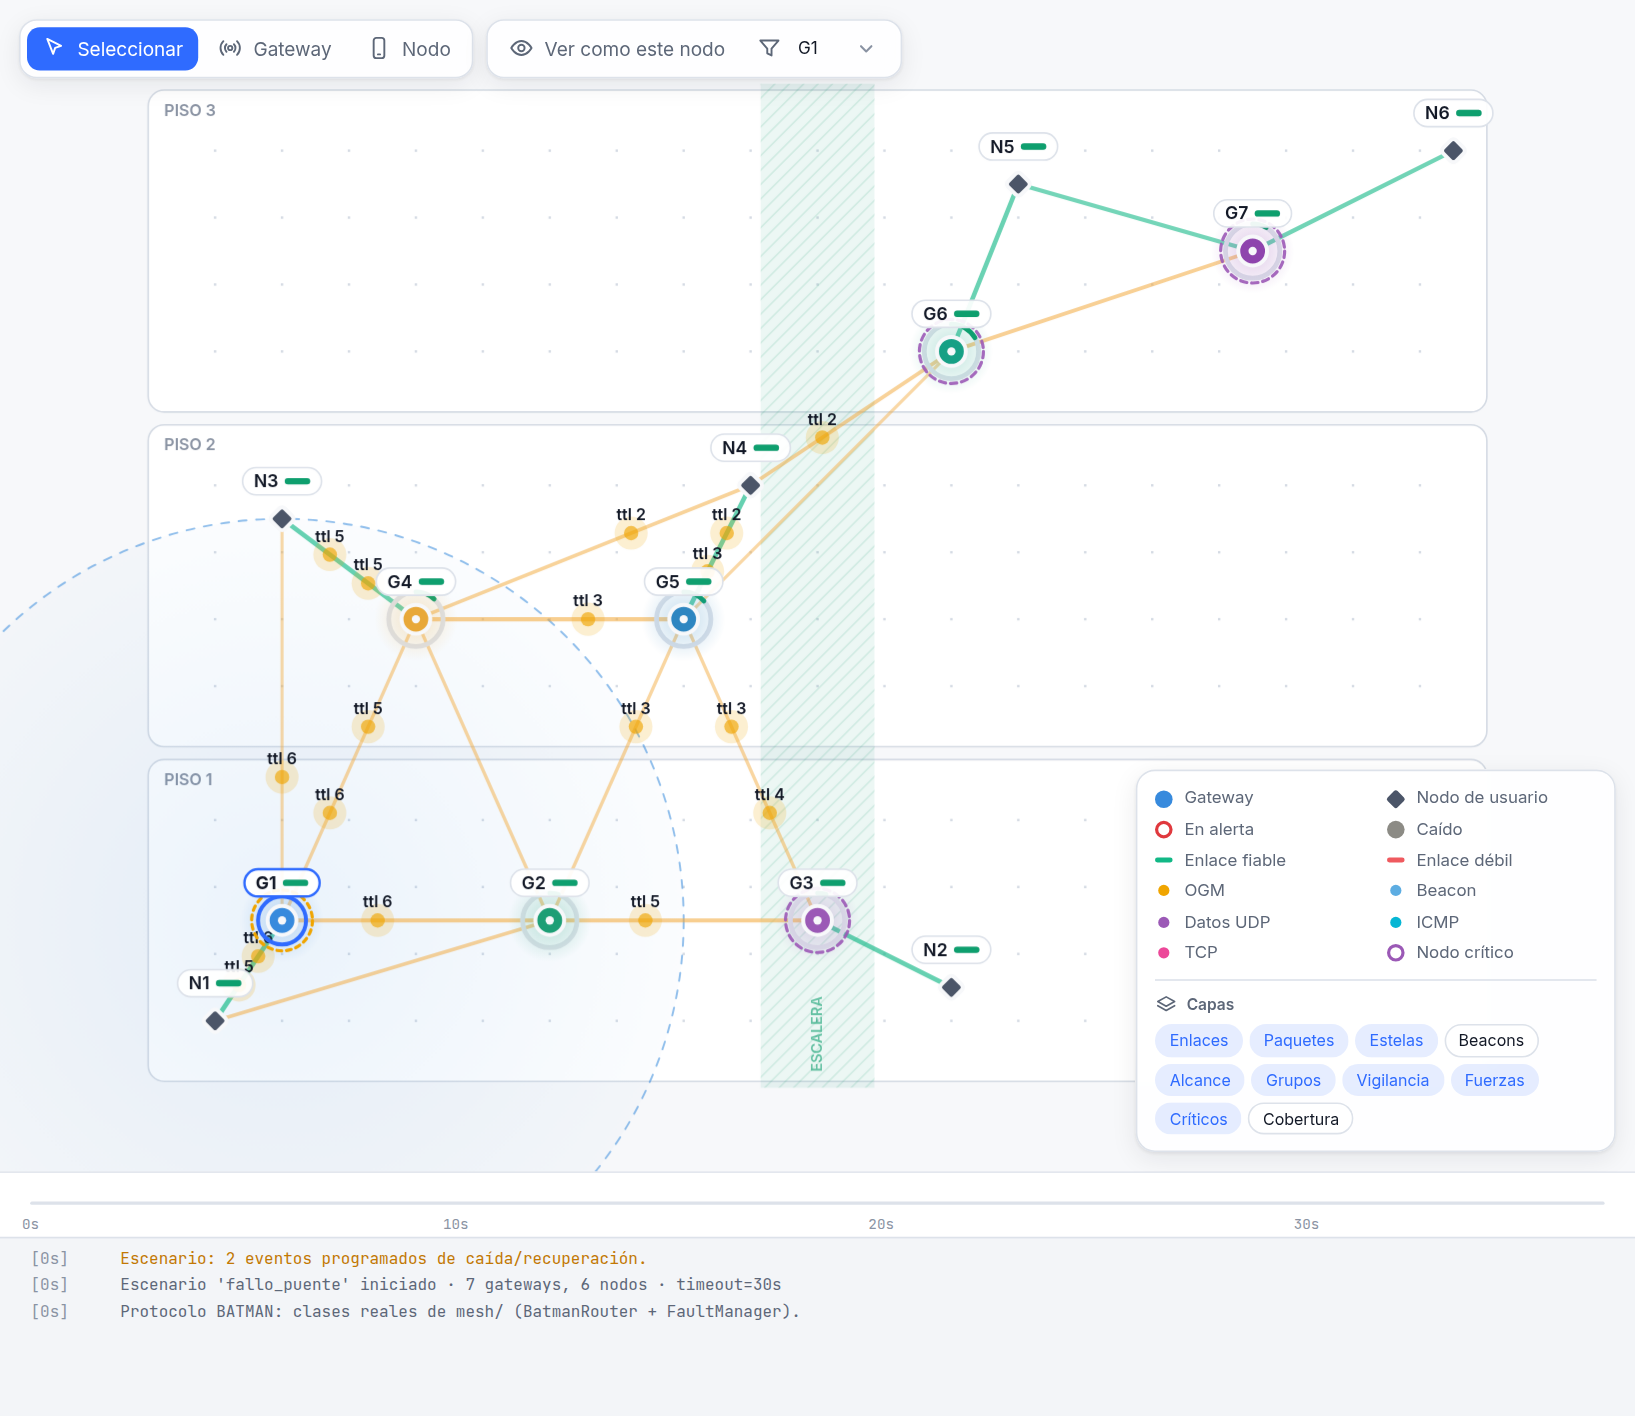
\includegraphics[width=0.92\textwidth]{Images/Cap4/ogm_propagacion.png}
    \caption{El protocolo en funcionamiento: propagación de los OGM originados por G1 (captura de la interfaz, escenario \texttt{fallo\_puente}, semilla 1). Cada punto naranja es una copia del mensaje viajando por un enlace, con el número de saltos que le quedan (``ttl''). Las copias cercanas a G1 llevan ttl 6 y 5; las que ya cruzaron varios nodos, ttl 3 y 2. El círculo punteado es el alcance de radio de G1}
    \label{fig:ogm}
\end{figure}

\textbf{Calidad de enlace y TQ.} Los enlaces de radio pierden mensajes. Para
saber qué tan bueno es un vecino, \texttt{BatmanRouter} lleva la cuenta de
cuántos de los últimos 16 OGM de cada origen le llegaron por ese vecino, como
en batman-adv~\cite{Seither2011BatmanAdv}. Con esa cuenta calcula la calidad del
enlace y la calidad de la ruta, según la Ecuación~(\ref{eq:tq}):
\begin{equation}
\label{eq:tq}
LQ_{o,v} = \frac{1}{|W_{o,v}|}\sum_{w\in W_{o,v}} w, \qquad TQ_{o,v} = TQ_{\text{OGM}} \cdot LQ_{o,v},
\end{equation}
donde:
\begin{itemize}
\item $o$ es el nodo que originó el OGM y $v$ es el vecino por el que llegó;
\item $W_{o,v}$ es la ventana de las últimas 16 secuencias de $o$ esperadas por
el vecino $v$, y $|W_{o,v}|$ es su tamaño;
\item $w$ es cada elemento de la ventana: vale 1 si esa secuencia se recibió y 0
si se perdió;
\item $LQ_{o,v}$ es la calidad del enlace: la fracción de OGM recibidos, entre 0
y 1;
\item $TQ_{\text{OGM}}$ es la calidad que trae escrita el mensaje, ya reducida por
cada nodo que lo reenvió;
\item $TQ_{o,v}$ es la calidad de la ruta hacia $o$ a través de $v$, entre 0 y 1.
\end{itemize}

\textbf{Elección de ruta.} Para cada destino, el nodo guarda el vecino con mejor
TQ. Otro vecino lo reemplaza solo si su TQ es mayor que el del actual, una vez
descontados los mensajes que el actual ha dejado de entregar.

\textbf{Detección de fallos.} Cada Gateway revisa cada 5~s, con
\texttt{FaultManager}, cuánto hace que no oye a los demás, y marca como caído al
que lleva más de 30~s en silencio. Nadie coordina esta revisión. Un mensaje
nuevo del nodo apaga la alerta.

\subsection{El modelo del medio de radiofrecuencia}
\label{sec:medio}

\texttt{RadioMedium} es lo único que reemplaza a la red real. Cada vez que un
nodo transmite, el modelo decide por separado, para cada nodo vivo, si el
mensaje le llega. Lo hace al azar, con la probabilidad de la
Ecuación~(\ref{eq:fiabilidad}), que se llama aquí \textit{fiabilidad} del enlace:
\begin{equation}
r(d,\Delta f) =
\begin{cases}
\max\!\big(0,\ \min\!\big(1,\ [\,1 - \phi\, d/R - p_0\,]\; a_f^{\,\Delta f}\big)\big) & \text{si } d \le R \\
0 & \text{si } d > R
\end{cases}
\label{eq:fiabilidad}
\end{equation}
donde:
\begin{itemize}
\item $r$ es la fiabilidad: la probabilidad, entre 0 y 1, de que una transmisión
llegue;
\item $d$ es la distancia entre los dos nodos, en metros;
\item $\Delta f$ es el número de pisos de diferencia entre los dos nodos;
\item $R$ es el alcance máximo del radio, en metros: más lejos no llega nada;
\item $\phi$ es la degradación con la distancia: cuánto baja la fiabilidad al
llegar al borde del alcance;
\item $p_0$ es la pérdida base: la fracción de mensajes que se pierde aun a
distancia cero;
\item $a_f$ es la atenuación por piso: el factor, entre 0 y 1, por el que se
multiplica la fiabilidad por cada piso de diferencia.
\end{itemize}

En palabras: la fiabilidad baja en línea recta con la distancia, se reduce por
cada piso que separa a los nodos y es cero fuera del alcance. Que cada piso
reste señal es un efecto medido en edificios
reales~\cite{Seidel1992Multifloor}. La Tabla~\ref{tab:parametros} muestra los
valores usados. El modelo es simple a propósito: es simétrico, no cambia en el
tiempo y no representa colisiones, supuestos que se saben
optimistas~\cite{Kotz2004Assumptions}. Lo que aporta frente a un simple dibujo
de conexiones es la pérdida entre pisos y que los mensajes perdidos hagan
variar el TQ. La distancia se mide en el corte vertical del edificio: es un
modelo de dos dimensiones con pisos, no una propagación en tres dimensiones.

\begin{table}[htbp!]
    \centering
    \caption{Valores de los parámetros del medio y del protocolo: los que el simulador trae por defecto, los del despliegue de referencia en el edificio y los del escenario de campo abierto}
    \label{tab:parametros}
    \footnotesize
    \begin{tabular}{|p{6.4cm}|p{1.8cm}|p{1.8cm}|p{2.2cm}|}
        \hline
        \textbf{Parámetro} & \textbf{Por defecto} & \textbf{Despliegue} & \textbf{Campo abierto} \\
        \hline
        Alcance de radio $R$ (m) & 16 & 12 & 30 \\
        \hline
        Degradación con la distancia $\phi$ & 0.85 & 0.5 & 0.6 \\
        \hline
        Pérdida base $p_0$ & 0.02 & 0.02 & 0.02 \\
        \hline
        Atenuación por piso $a_f$ & 0.55 & 0.8 & no aplica \\
        \hline
        Tiempo límite de detección (s) & 30 & 30 & 30 \\
        \hline
        Periodo de \textit{beacons} / de OGM (s) & 2 / 4 & 2 / 4 & 2 / 4 \\
        \hline
        Velocidad de un Gateway (m por paso) & 0.32 & 0 (fijos) & 0.6 \\
        \hline
    \end{tabular}
\end{table}

\subsection{Envío de paquetes de datos}
\label{sec:plano-datos}

En el simulador de partida, un mensaje se entregaba buscando el camino en la
red real, y llegaba siempre que existiera alguno. Las tablas de rutas no
decidían nada. En este diseño, cada paquete avanza salto a salto: en cada nodo,
el siguiente salto lo decide \texttt{BatmanRouter.next\_hop()} con la tabla de
ese nodo. Nadie conoce el camino completo. Cada salto es un envío dirigido a un
solo vecino, que se reintenta hasta 3 veces si se pierde. La capa de enlace de
las redes inalámbricas también reenvía las tramas que no se confirman, con sus
propios límites de reintento~\cite{IEEE80211}; el valor de 3 es una
simplificación de este simulador. Un paquete que da más de 50
saltos se descarta.

Así, un paquete puede perderse aunque exista un camino, y la causa queda
registrada. Las pérdidas se separan en físicas (el destino está caído o no hay
ningún camino por radio) y de enrutamiento (el nodo no tiene ruta, la ruta
apunta a un vecino que ya no está al alcance, el radio perdió el salto o el
paquete quedó dando vueltas en un bucle). Esta separación permite no culpar al
protocolo de lo que es física. Cada salto se resuelve dentro del mismo paso,
porque un salto real dura mucho menos que 0.5~s; por eso el simulador no mide el
retardo.

\textbf{Tipos de paquete.} El usuario elige qué tipo de paquete se envía,
cuántos y cada cuánto tiempo. Los tres tipos usan el mismo avance salto a
salto y se diferencian en lo que ocurre entre el origen y el destino:

\begin{itemize}
\item \textbf{UDP}~\cite{Postel1980UDP}: un paquete de ida, sin confirmación. Si
se pierde, nadie lo vuelve a enviar.
\item \textbf{ICMP}~\cite{Postel1981ICMP}: un eco, como la orden \texttt{ping}.
La petición va y el destino responde, usando su propia tabla de rutas para el
regreso. Cuenta como entregado solo si la respuesta vuelve al origen.
\item \textbf{TCP}~\cite{Eddy2022TCP}: el destino confirma cada paquete y el
origen lo vuelve a enviar, hasta 3 veces, si la confirmación no llega.
\end{itemize}

Son versiones simplificadas de esos protocolos: no hay establecimiento de
conexión ni control de congestión, y los reenvíos de TCP ocurren dentro del
mismo paso, de modo que solo recuperan pérdidas del radio.

\subsection{Movimiento descentralizado de los Gateway}
\label{sec:movilidad-descentralizada}

El simulador tiene tres modos de movimiento de los Gateway. Dos deciden con
información global y se conservan solo como referencia: \textit{seguir} lleva a
cada Gateway hacia el usuario más cercano mirando las posiciones de todos, y
\textit{repartir} asigna un usuario distinto a cada Gateway desde el motor del
simulador.

En el modo \textit{descentralizado}, cada Gateway decide únicamente con lo que
oyó en los \textit{beacons} de sus vecinos, que llevan la posición de quien los
emite. Esto supone que cada nodo conoce su posición, por ejemplo con un sistema
de localización, como es habitual en estos
métodos~\cite{Howard2002PotentialFields}. Si pasa 3 periodos sin oír a un
vecino, lo olvida. La decisión combina cuatro reglas, de la familia de las
``fuerzas virtuales'' revisadas en la
Sección~\ref{sec:redes-desastre}~\cite{Howard2002PotentialFields,Zou2003VirtualForces,Poduri2004ConstrainedCoverage},
con distancias expresadas como fracción del alcance $R$:

\begin{itemize}
\item \textbf{Cobertura.} El Gateway se acerca a los usuarios que oye y de los
que es el Gateway más cercano, si están a más de $0.4R$.
\item \textbf{Separación.} Se aleja de los Gateway que oye a menos de $0.55R$,
para no amontonarse.
\item \textbf{Expansión.} Si no tiene usuarios a su cargo, se aleja de los demás
hasta $0.75R$: la malla se estira hasta oír usuarios nuevos.
\item \textbf{Reconexión.} Si no oye a ningún Gateway, vuelve hacia el último
que oyó.
\end{itemize}

A estas reglas se suma una de seguridad: un Gateway no da un paso que rompa el
enlace con otro Gateway que oye, salvo que quede un camino de dos saltos a
través de un tercero. Como la posición que trae un \textit{beacon} puede tener
varios segundos, el Gateway supone que el vecino pudo haberse movido y solo
considera seguro un enlace si lo es en el peor caso. La
Figura~\ref{fig:fuerzas} muestra el movimiento descentralizado en la interfaz.

Los umbrales se eligieron probando combinaciones sobre cuatro escenarios, con 5
semillas. Esa búsqueda dejó dos aprendizajes. Sin la regla de expansión, los
Gateway que arrancan juntos y no oyen a nadie se quedan quietos: en el escenario
\texttt{base} la cobertura era de 0.23. Y recordar a los vecinos por más tiempo
empeoraba las particiones, porque las posiciones viejas engañan más de lo que
ayudan.

\subsection{Medir lo que cree cada nodo}
\label{sec:metricas-descentralizacion}

Para cada par de nodos vivos, el simulador compara en cada muestra lo que cree
el primero (si tiene una ruta vigente hacia el segundo) con la realidad (si el
radio los conecta). De ahí salen la exactitud del conocimiento y las rutas
fantasma y faltantes de la Tabla~\ref{tab:metricas}. Una ruta es
\textit{vigente} si un OGM la refrescó hace menos que el tiempo límite.

Un \textit{nodo crítico} es aquel cuya caída parte la red en dos o más grupos.
Se calculan con el algoritmo de puntos de articulación de un
grafo~\cite{Hopcroft1973Algorithm447}. Con esa base se diseñaron dos tipos de
caída que eligen al nodo en el momento del fallo: \textit{al azar} y
\textit{dirigida}, que tumba al nodo que más nodos deja aislados. Esto permite
comparar un fallo cualquiera con el peor fallo posible, como en los estudios de
errores y ataques en redes~\cite{Albert2000ErrorAttack}.

\subsection{Otros mapas, otros movimientos y un protocolo de comparación}
\label{sec:generalidad}

Para que la herramienta no quede atada al edificio de partida, el diseño
incluye:

\begin{itemize}
\item \textbf{Mapa de campo abierto:} un área vista desde arriba, sin pisos. El
escenario \texttt{campo\_abierto} mide 120~$\times$~80~m y tiene 6 Gateway que
salen del mismo punto, 9 usuarios en 3 grupos y 6 flujos de datos.
\item \textbf{Movimiento de los usuarios:} además de usuarios quietos, pueden
caminar hacia puntos al azar (\textit{random
waypoint}~\cite{Camp2002MobilitySurvey}) o moverse en grupos (inspirado en el
modelo RPGM~\cite{Hong1999GroupMobility}).
\item \textbf{Protocolo de comparación:} en la \textit{inundación}, cada nodo
repite una vez cada paquete nuevo a todos sus vecinos, sin tablas de rutas ni
reintentos~\cite{Ni1999BroadcastStorm}.
\item \textbf{Parámetros en un solo lugar:} cualquier parámetro del medio o del
protocolo se puede cambiar desde la terminal, un lote o la interfaz.
\end{itemize}

% ════════════════════════════════════════════════════════════════════════
\section{Implementación}
\label{sec:implementacion}

El simulador está escrito en el lenguaje Python~\cite{Python}. Para los
cálculos y las figuras usa las bibliotecas NumPy~\cite{Harris2020Numpy} y
Matplotlib~\cite{Hunter2007Matplotlib}, y para la ventana propia,
pygame-ce~\cite{PygameCe}. La
interfaz web usa solo lo que trae Python y páginas que el navegador abre sin
instalar nada más.

\subsection{Escenarios, lotes y formas de ejecución}
\label{sec:ejecucion}

Un escenario es un archivo de texto que describe el medio, el protocolo, los
nodos, los eventos y el tráfico. Al cargarlo, el simulador lo revisa y rechaza
con un mensaje claro los errores, como identificadores repetidos o posiciones
fuera del mapa. Este es un fragmento del escenario de la caída del puente, con
un flujo de tráfico añadido como ejemplo:

\begin{verbatim}
[medium]
rango_comm=12        # alcance R, en metros
falloff=0.5          # degradación con la distancia
floor_atten=0.8      # atenuación por piso

[nodes]
# id  rol  x   y   (G = Gateway, N = usuario)
1    G    4   5
...
6    G    24  22
101  N    2   2

[events]
fail     6  60       # el nodo 6 se cae a los 60 s
recover  6  150      # y vuelve a los 150 s

[traffic]
# origen destino cada(s) tipo cantidad
101  104  1  tipo=icmp cantidad=20
\end{verbatim}

La misma simulación se puede ejecutar de cuatro formas: en una ventana propia;
sin ventana, con el resumen en la terminal; por lotes, que repiten varios
escenarios con varias semillas y calculan el promedio; y en la interfaz web.
Las cuatro construyen la simulación con la misma función, de modo que dan los
mismos números.

\subsection{Interfaz web}
\label{sec:interfaz}

La interfaz se abre con \texttt{python main.py --web}, funciona sin conexión a
Internet y la atiende el mismo programa del simulador. El navegador solo dibuja
lo que recibe: la fiabilidad, las rutas y las métricas se calculan en el
simulador, de modo que no hay una segunda versión de los cálculos que pueda dar
otro resultado. Esta sección muestra cada función de la interfaz con una
captura tomada del simulador en funcionamiento. Todas las capturas son de
elaboración propia.

\textbf{Vista general.} La Figura~\ref{fig:interfaz} muestra la pantalla
completa durante la prueba de la caída del puente. A la izquierda está el mapa
del edificio con los nodos y sus enlaces; arriba, los controles de tiempo y el
estado de la red; a la derecha, el panel del nodo seleccionado, con su tabla de
rutas; abajo, la línea de tiempo y el registro de lo que va ocurriendo.

\begin{figure}[htbp!]
    \centering
    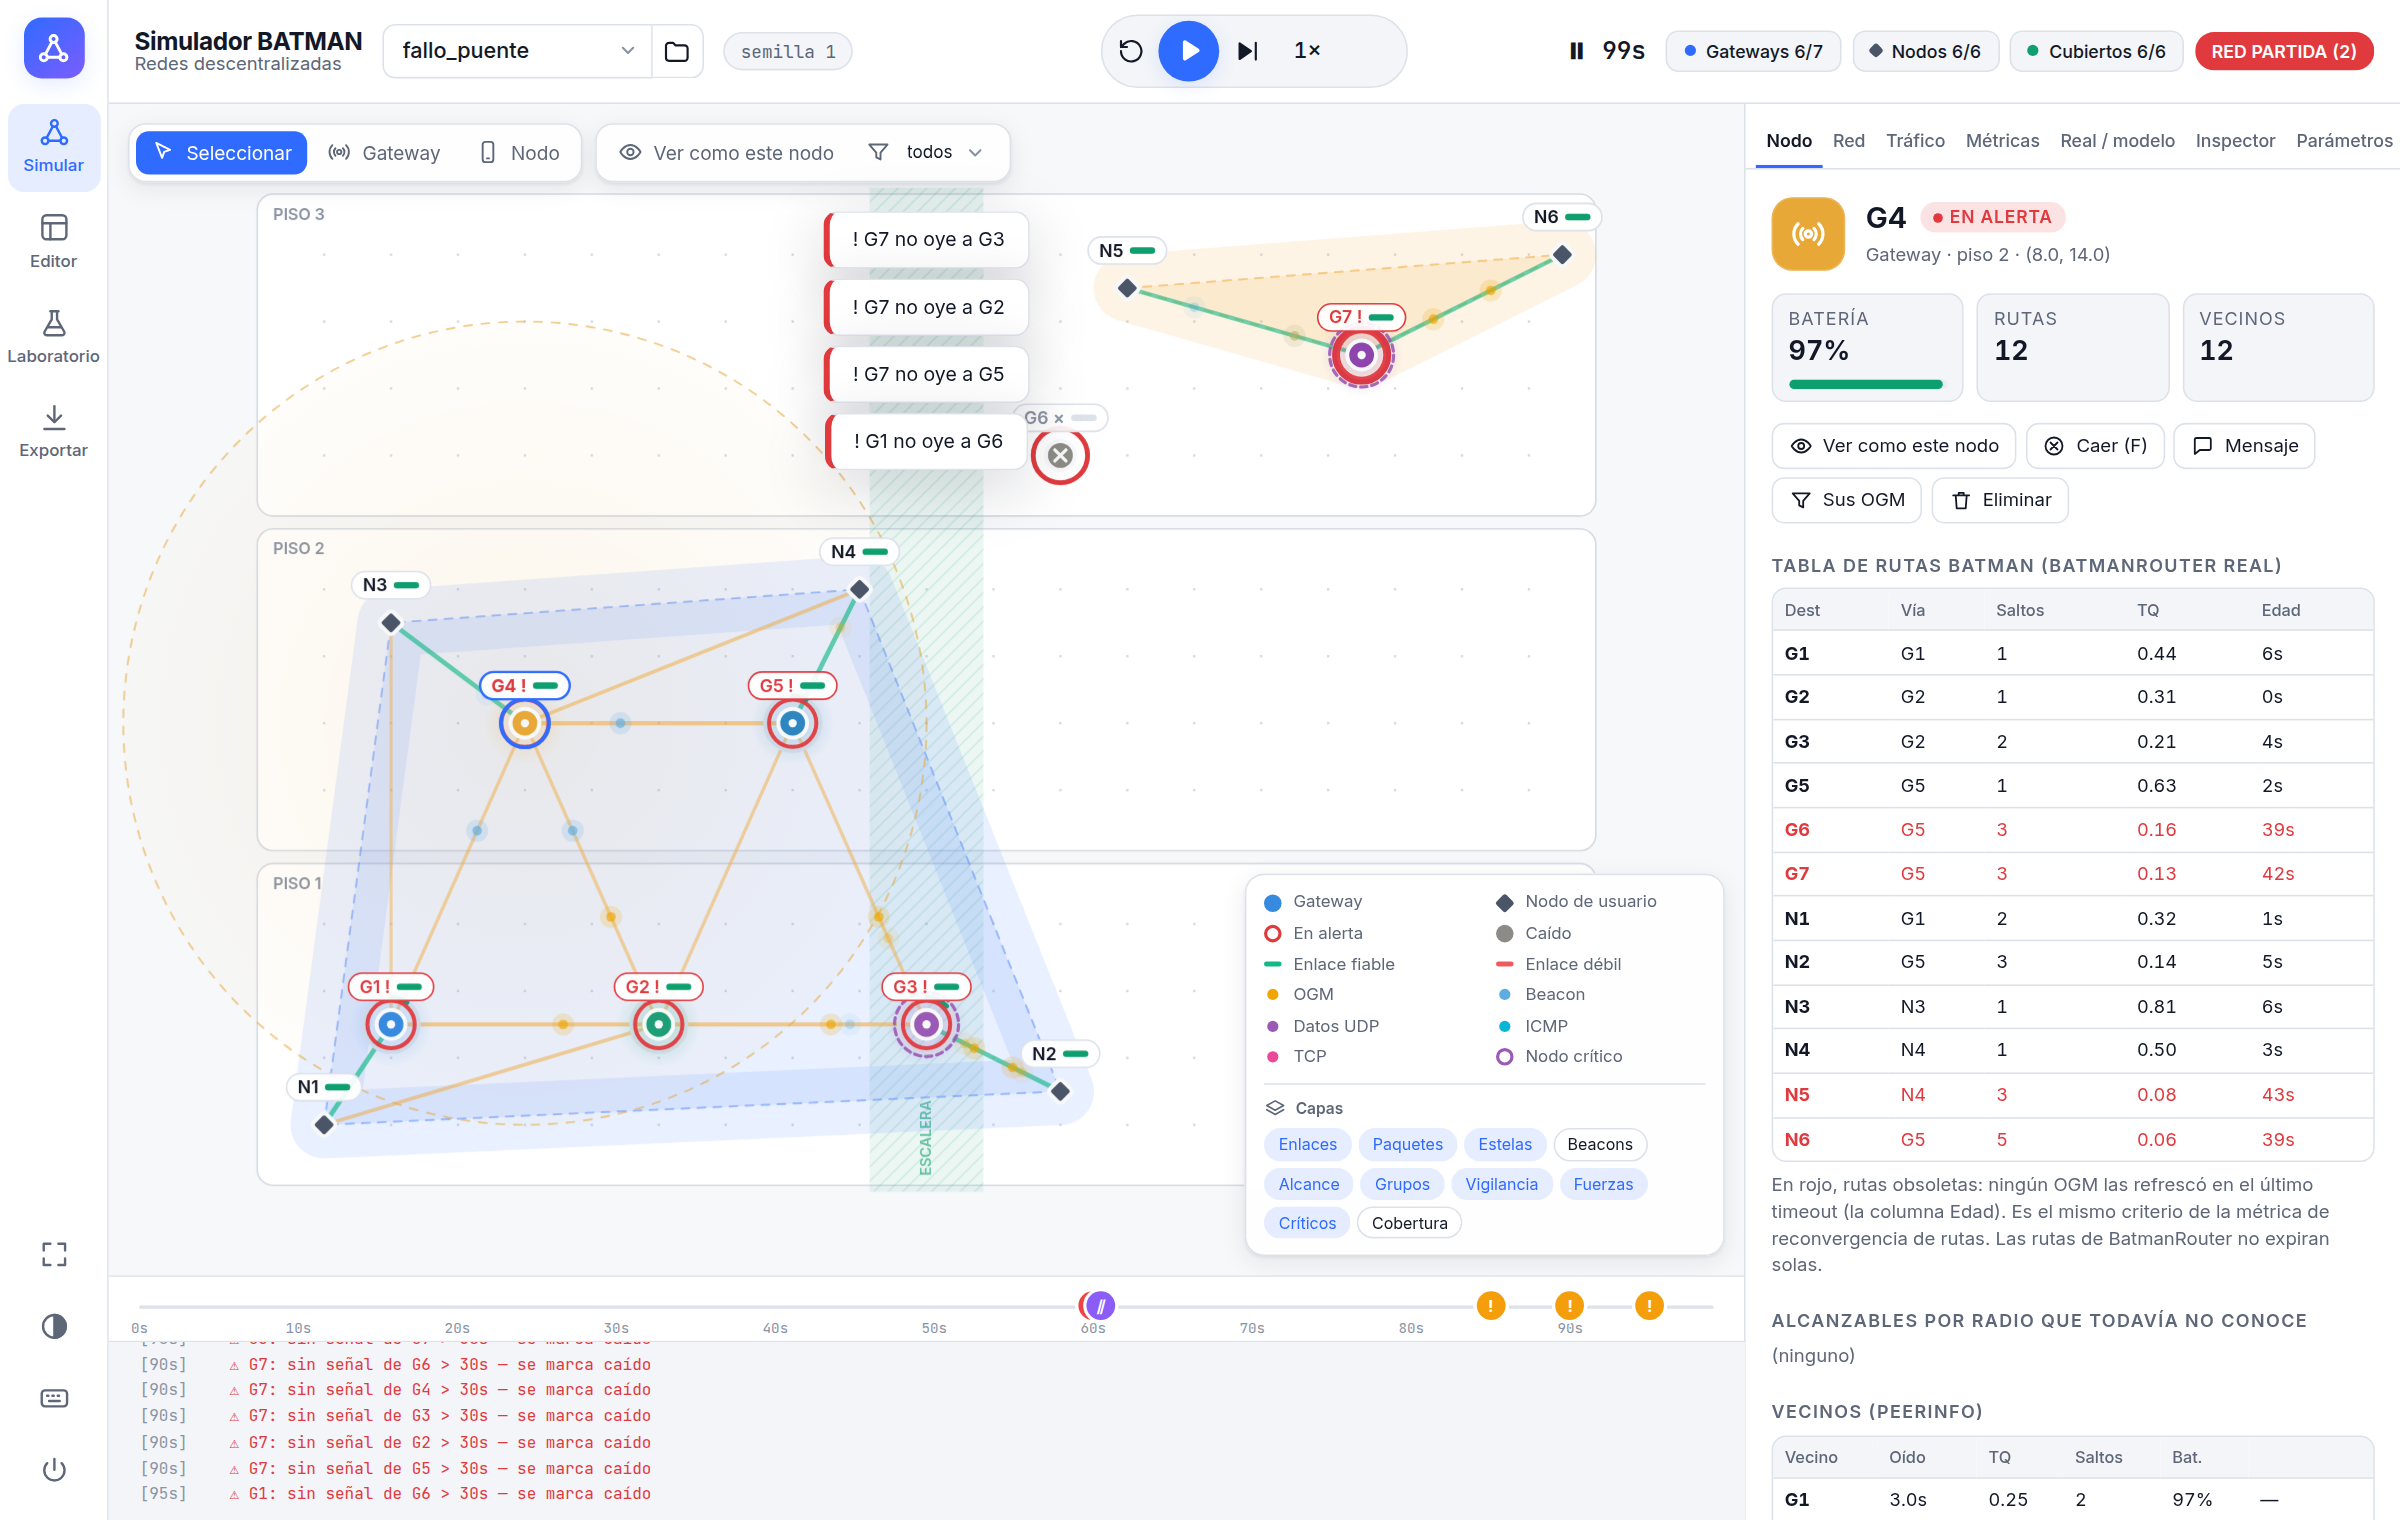
\includegraphics[width=\textwidth]{Images/Cap4/interfaz_fallo_puente.png}
    \caption{Vista general de la interfaz a los 99~s de la prueba de la caída del puente (semilla 1). En el mapa, G6 aparece caído (círculo gris con una equis) y las dos zonas sombreadas son los dos grupos en que quedó partida la malla. Arriba a la derecha, el aviso rojo ``Red partida (2)'' y el indicador ``Cubiertos 6/6'': los seis usuarios siguen cubiertos. Los Gateway con borde rojo tienen alertas activas. A la derecha, la tabla de rutas de G4: en rojo, las rutas hacia el piso 3 que ya nadie refresca}
    \label{fig:interfaz}
\end{figure}

\textbf{Lo que sabe un nodo.} El panel de nodo (a la derecha en la
Figura~\ref{fig:interfaz}) muestra la tabla de rutas del nodo: para cada
destino, por cuál vecino enviar, a cuántos saltos está, con qué calidad y hace
cuánto se refrescó. La función ``Ver como este nodo''
(Figura~\ref{fig:lente}) redibuja el mapa solo con lo que sabe el nodo elegido.

\begin{figure}[htbp!]
    \centering
    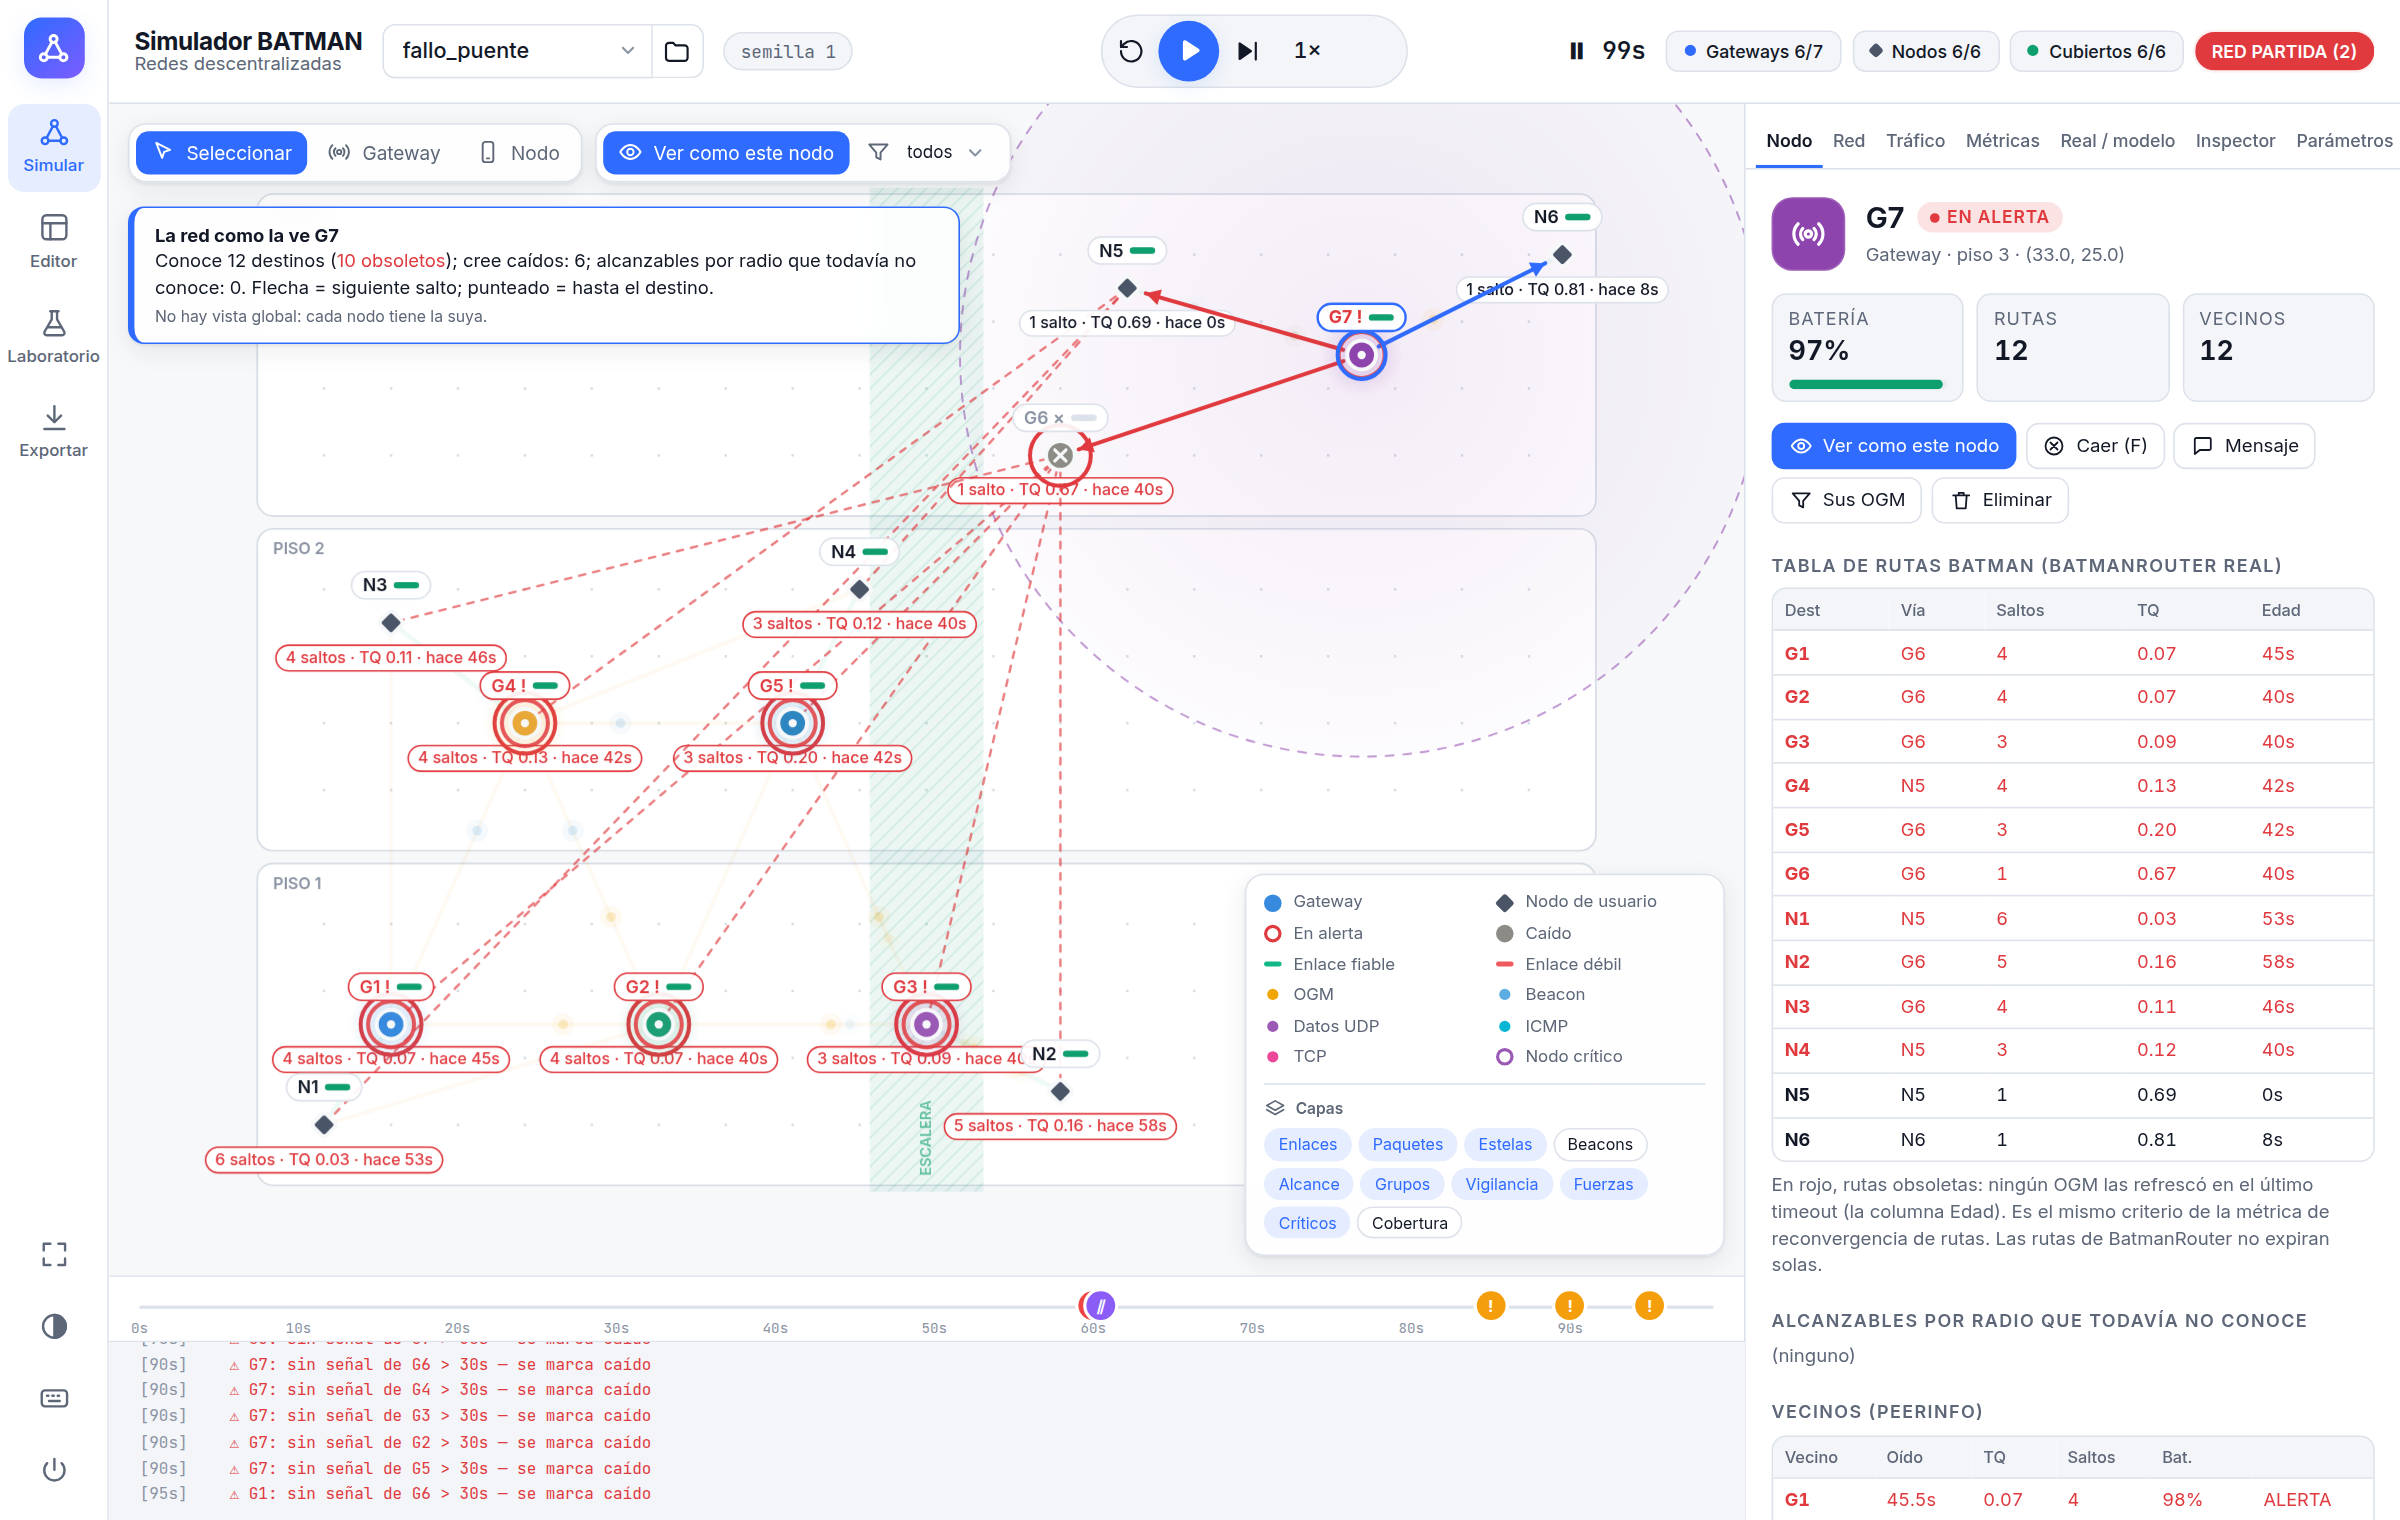
\includegraphics[width=\textwidth]{Images/Cap4/lente.png}
    \caption{Función ``Ver como este nodo'', aplicada a G7 a los 99~s de la prueba de la caída del puente. El mapa solo muestra lo que G7 sabe: las flechas continuas son sus rutas vigentes (hacia N5 y N6) y las líneas punteadas rojas son rutas que conserva en su tabla hacia nodos que ya no puede alcanzar, con los saltos, la calidad y la antigüedad de cada una. El recuadro superior resume cuántos destinos conoce y cuántos están obsoletos}
    \label{fig:lente}
\end{figure}

\textbf{Lo que sabe toda la red.} La matriz de conocimiento
(Figura~\ref{fig:matriz}) reúne en una cuadrícula lo que sabe cada nodo sobre
cada uno de los demás, y permite ver de un vistazo si la red ya se conoce a sí
misma y qué rutas quedan después de una partición.

\begin{figure}[htbp!]
    \centering
    \begin{subfigure}{0.49\textwidth}
        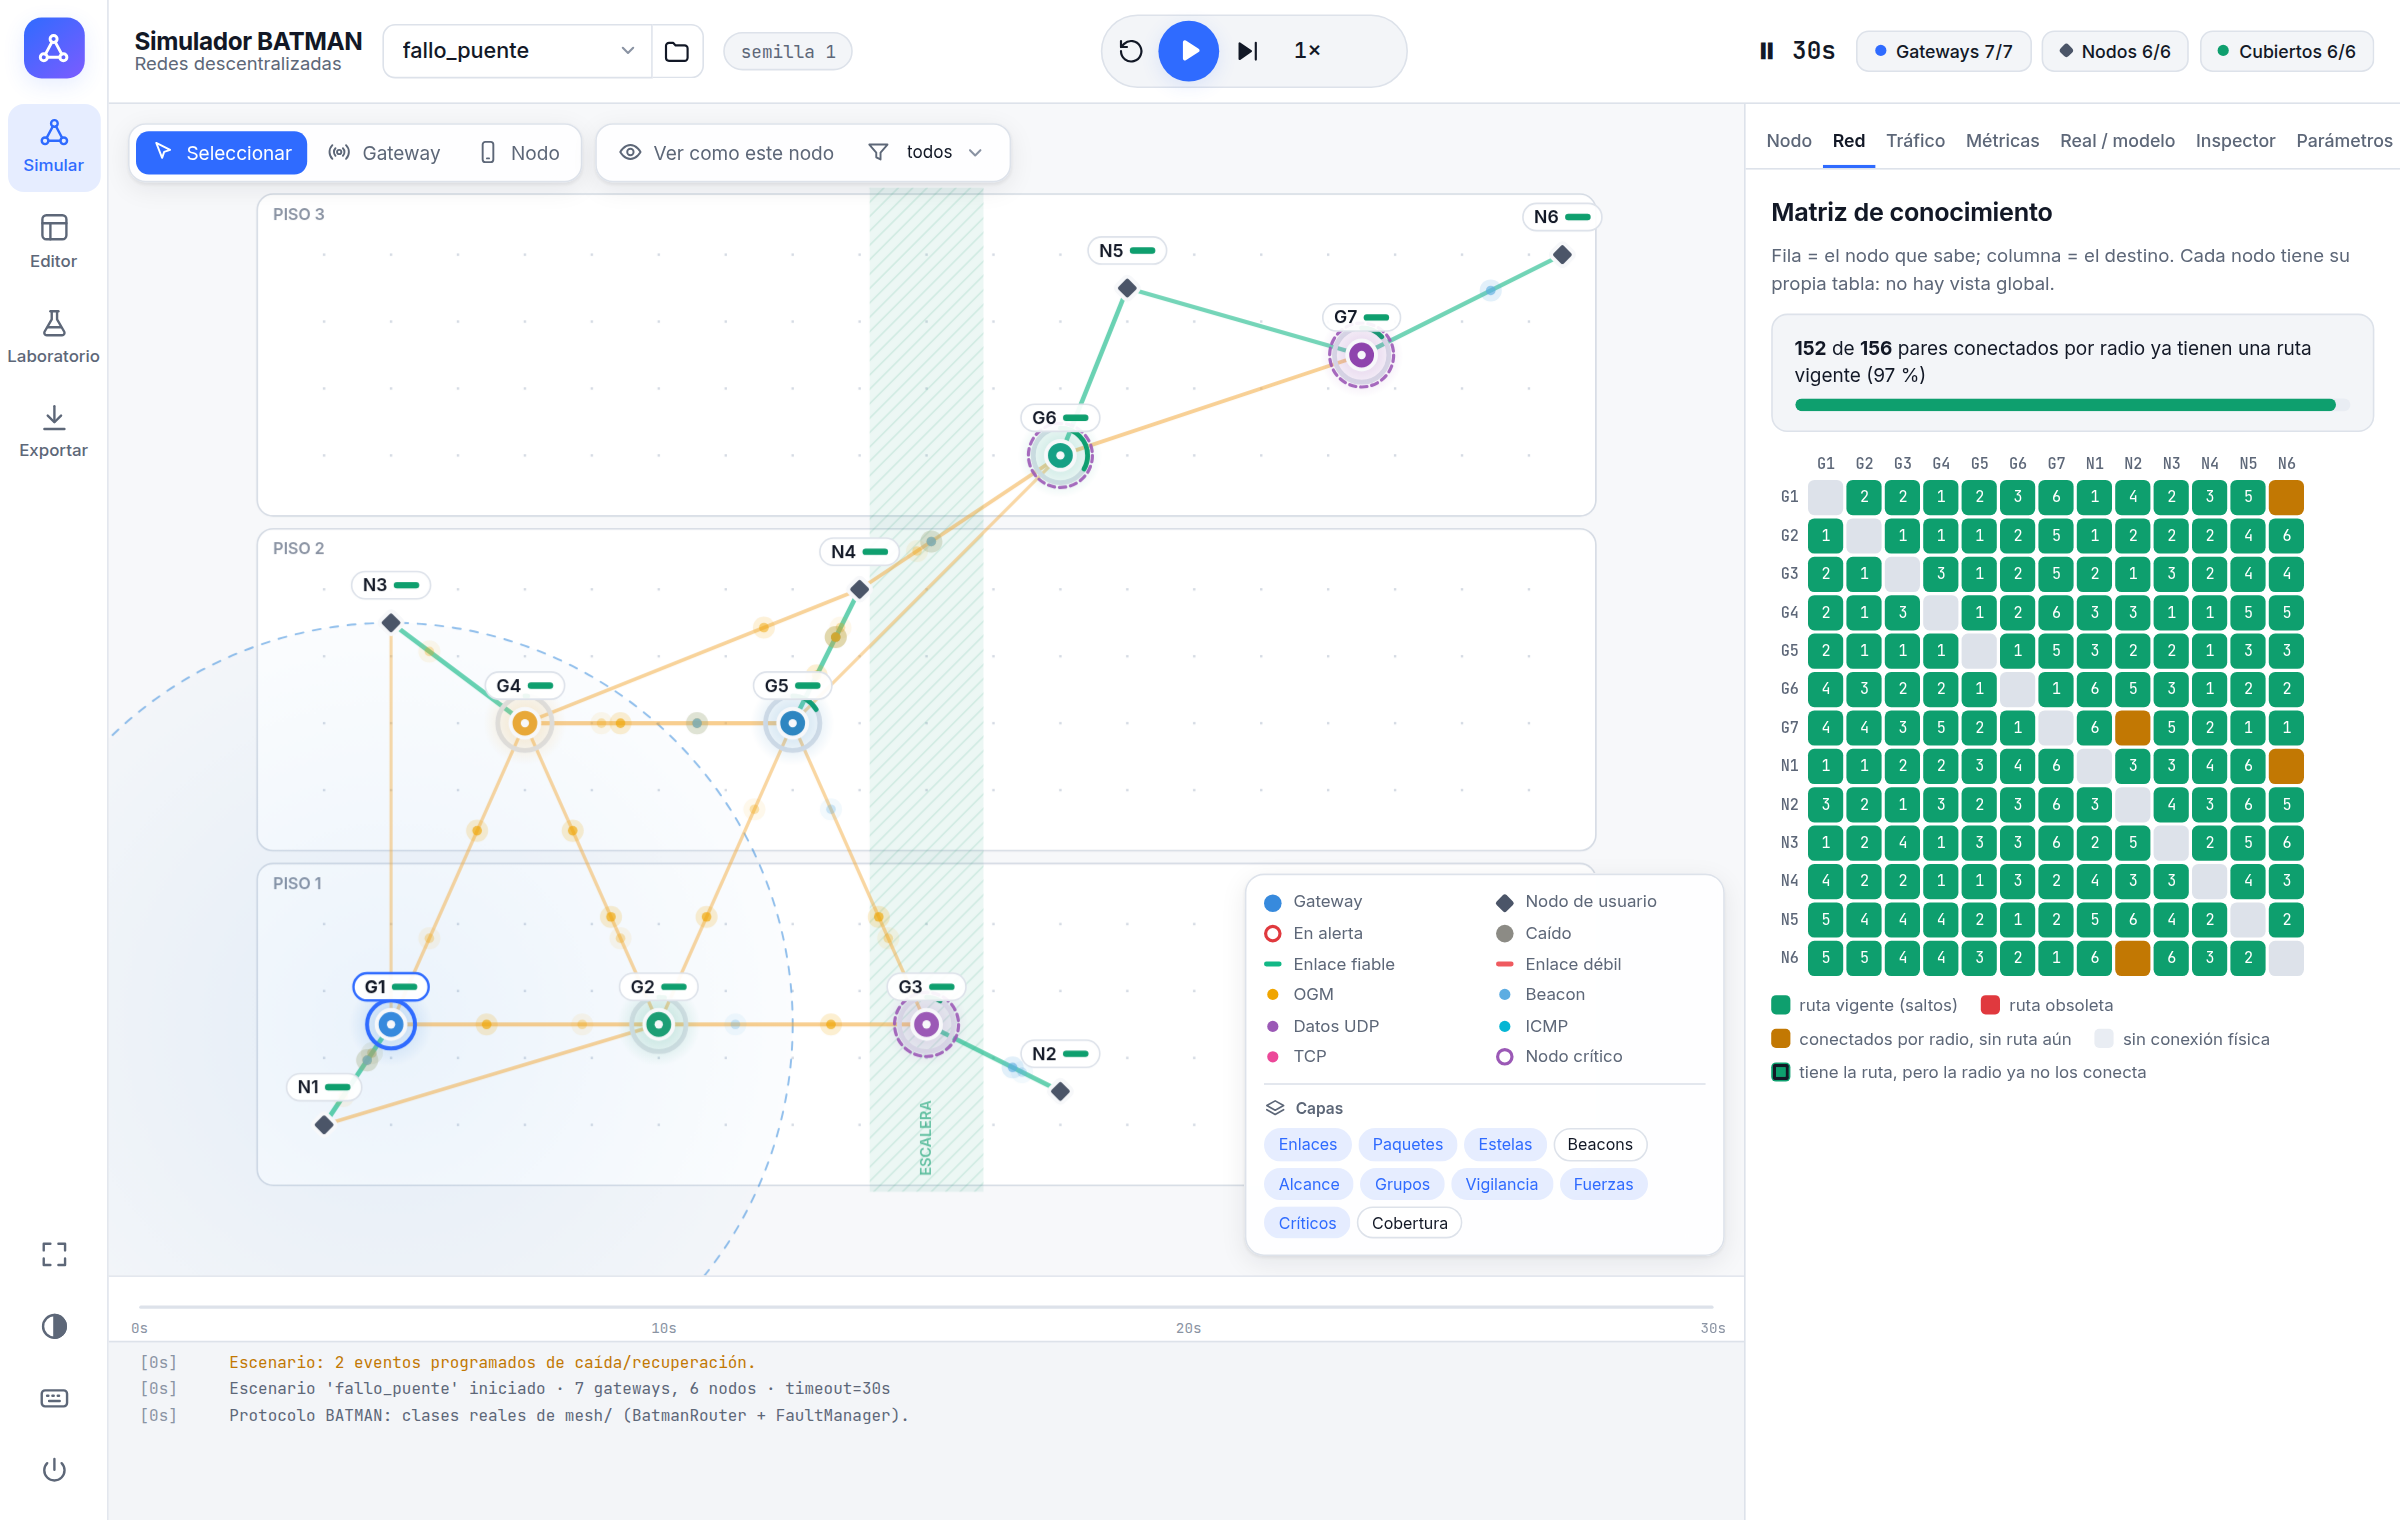
\includegraphics[width=\textwidth, trim=1740 250 0 130, clip]{Images/Cap4/matriz_formada.png}
        \caption{A los 30~s, antes del fallo}
    \end{subfigure}\hfill
    \begin{subfigure}{0.49\textwidth}
        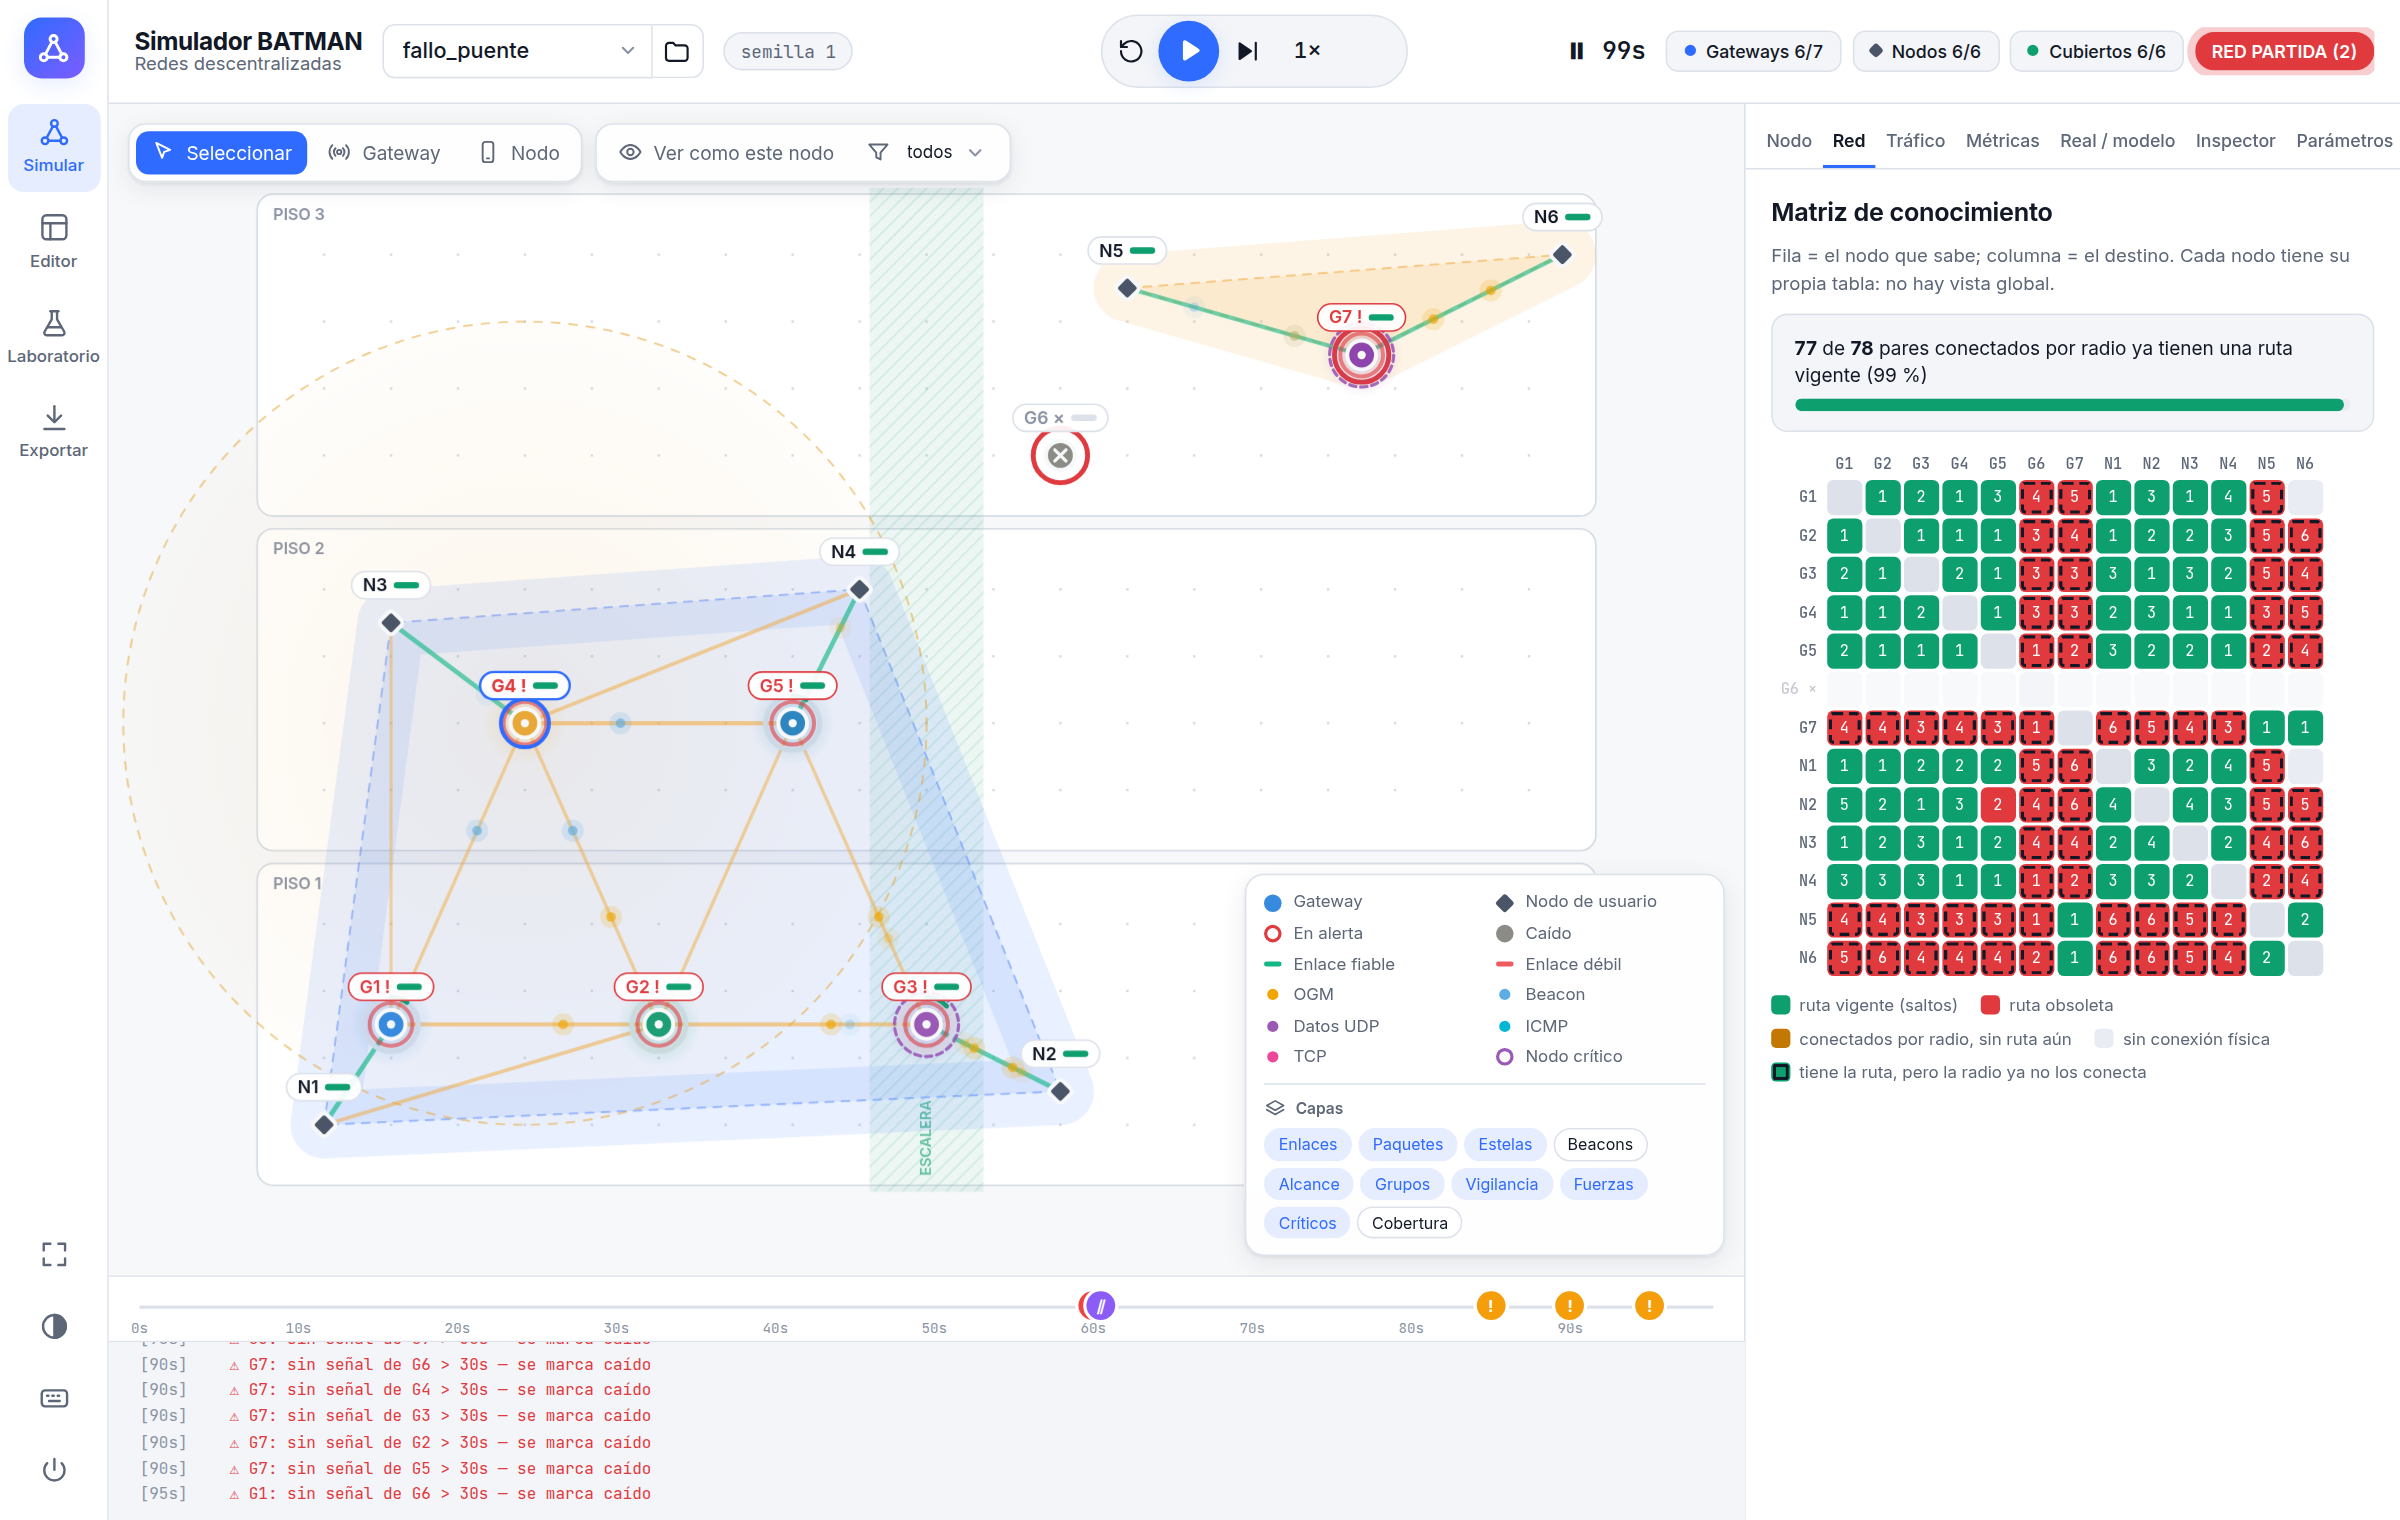
\includegraphics[width=\textwidth, trim=1740 250 0 130, clip]{Images/Cap4/matriz_particion.png}
        \caption{A los 99~s, con el puente caído}
    \end{subfigure}
    \caption{Matriz de conocimiento. Cada fila es un nodo que ``sabe'' y cada columna, un destino. Una casilla verde es una ruta vigente, con su número de saltos; una naranja, un par conectado por radio que todavía no tiene ruta; una roja, una ruta obsoleta. (a) Con la malla formada, 152 de los 156 pares conectados por radio ya tienen ruta (97~\%). (b) Con G6 caído, las rutas entre el piso 3 y el resto aparecen en rojo: siguen en las tablas, pero ya no sirven}
    \label{fig:matriz}
\end{figure}

\textbf{Qué es real y qué es modelo.} El panel de la
Figura~\ref{fig:real-modelo} atiende el requerimiento R2: separa lo que hizo el
código del nodo (mensajes procesados, rutas, revisiones de fallos) de lo que
aportó el modelo (transmisiones intentadas y entregadas por el medio).

\begin{figure}[htbp!]
    \centering
    \begin{subfigure}{0.49\textwidth}
        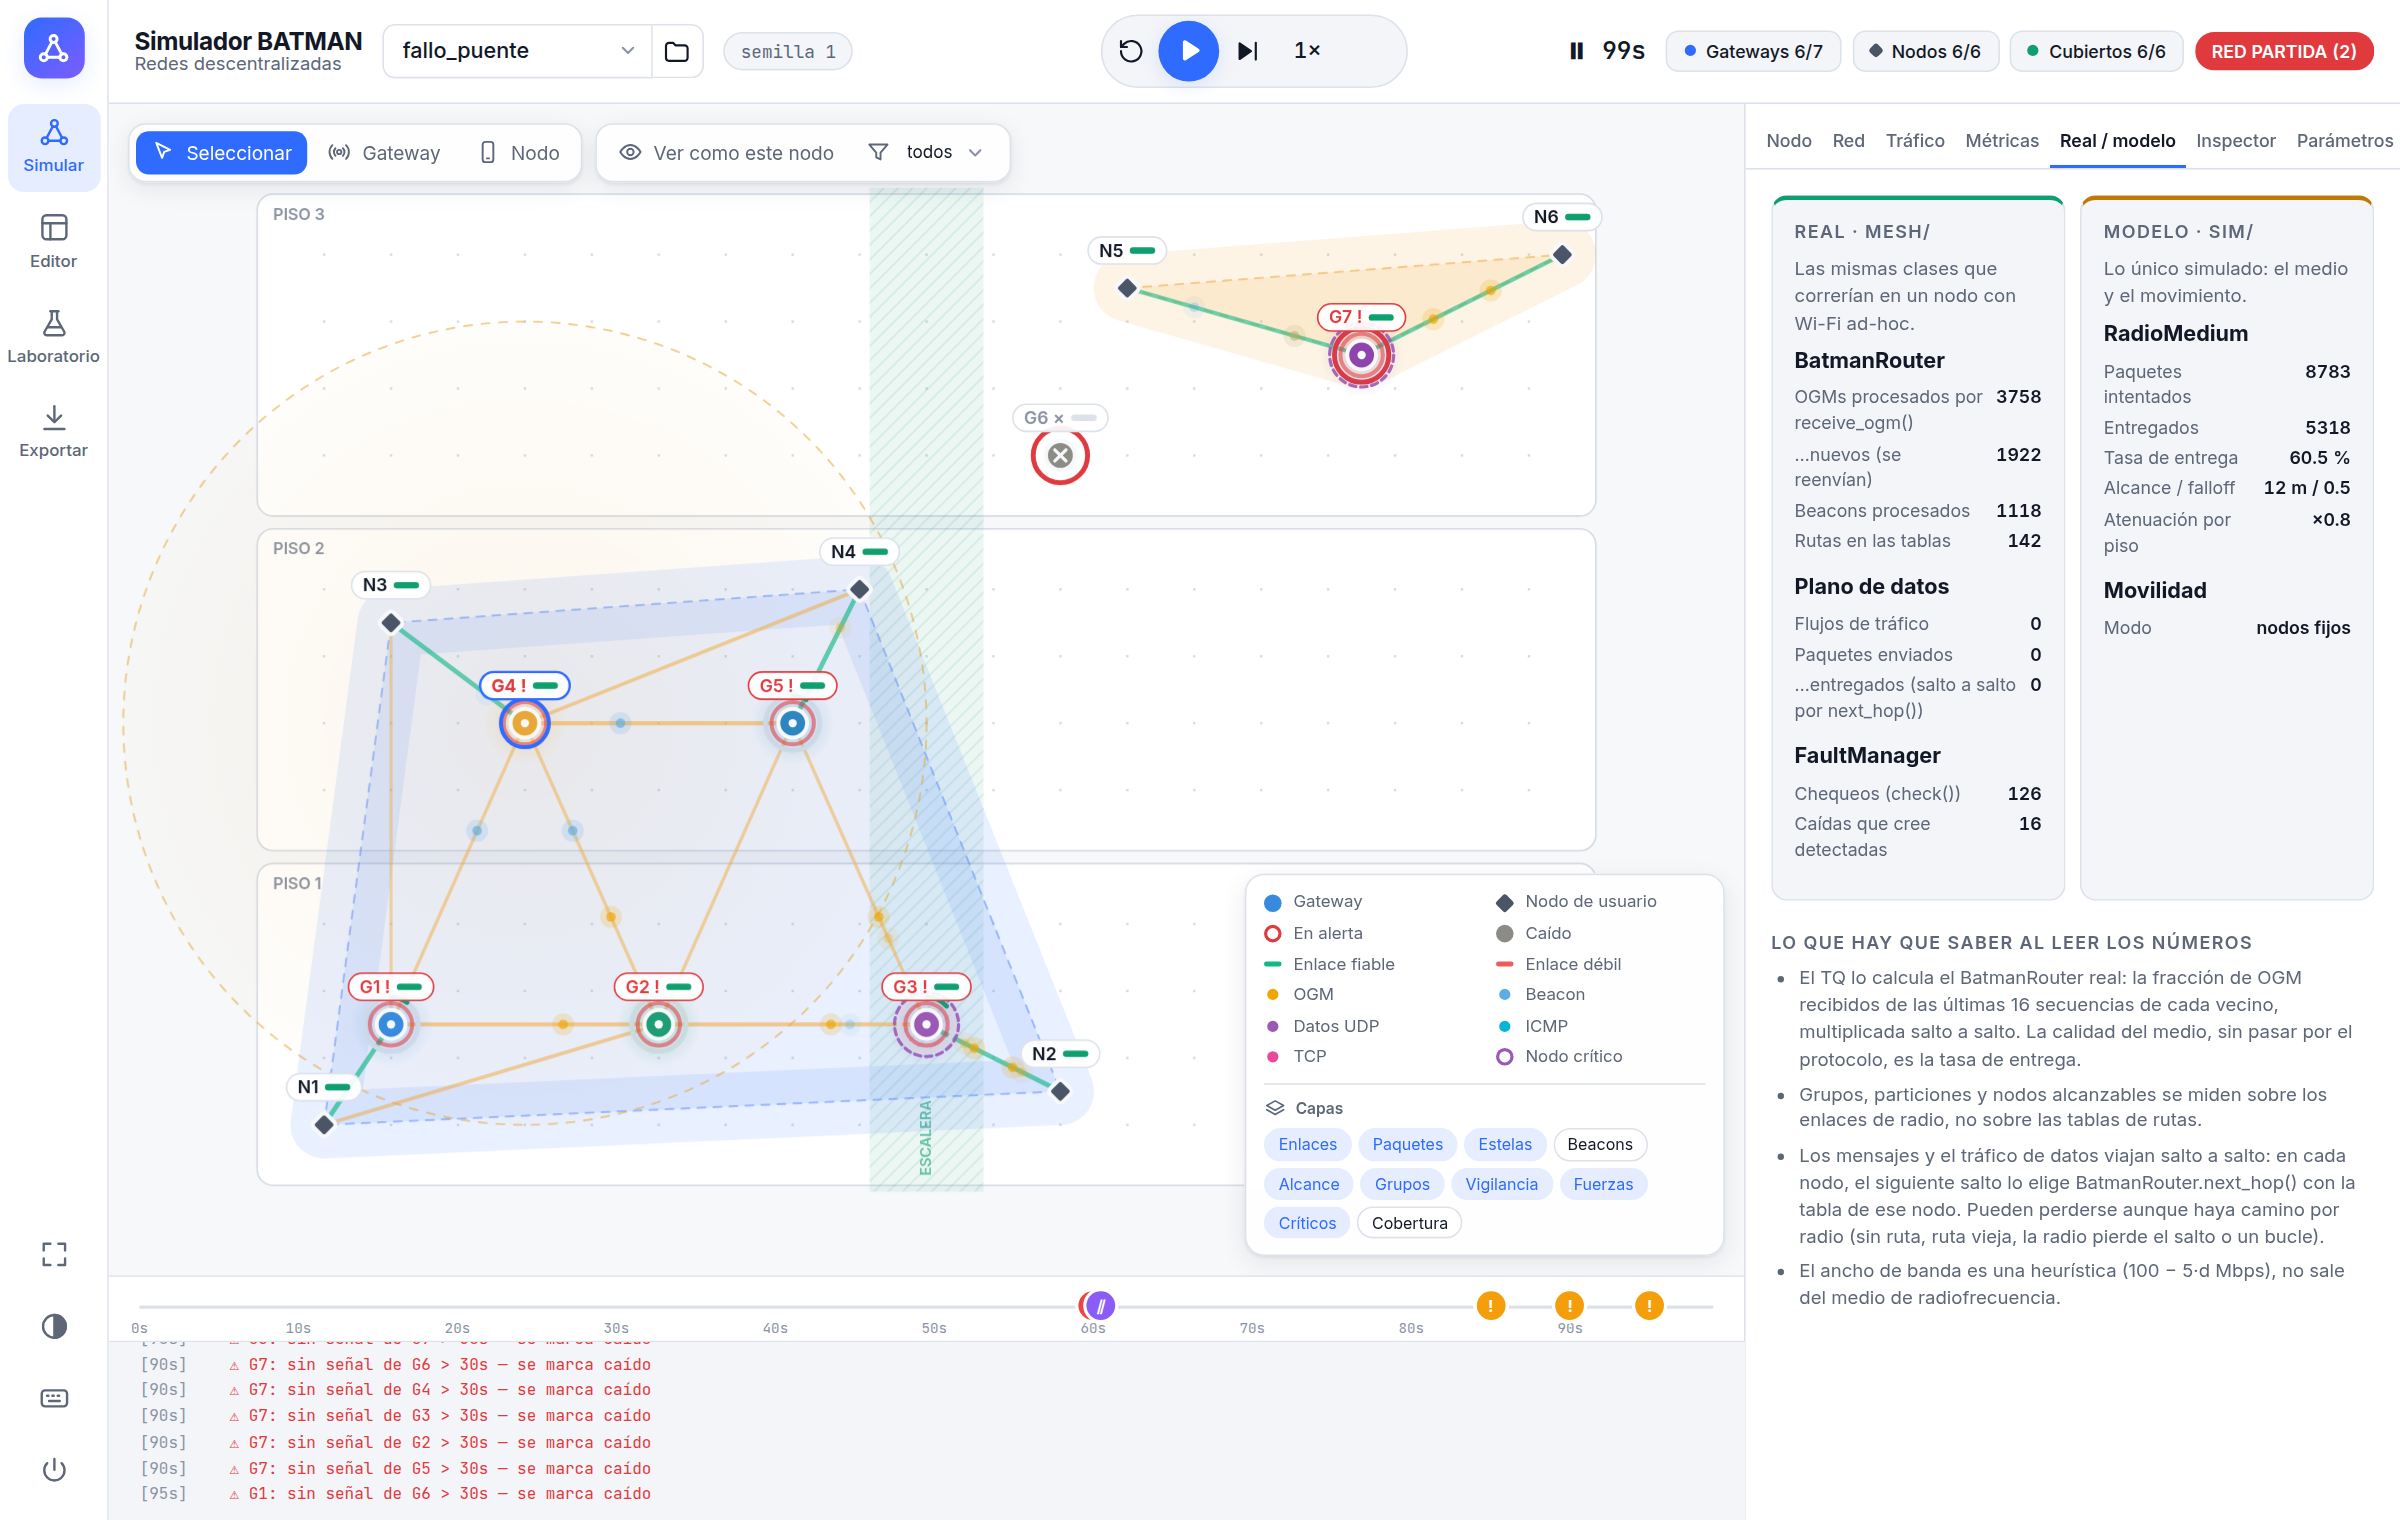
\includegraphics[width=\textwidth, trim=1740 250 0 130, clip]{Images/Cap4/real_modelo.png}
        \caption{Panel ``Real / modelo''}
    \end{subfigure}\hfill
    \begin{subfigure}{0.49\textwidth}
        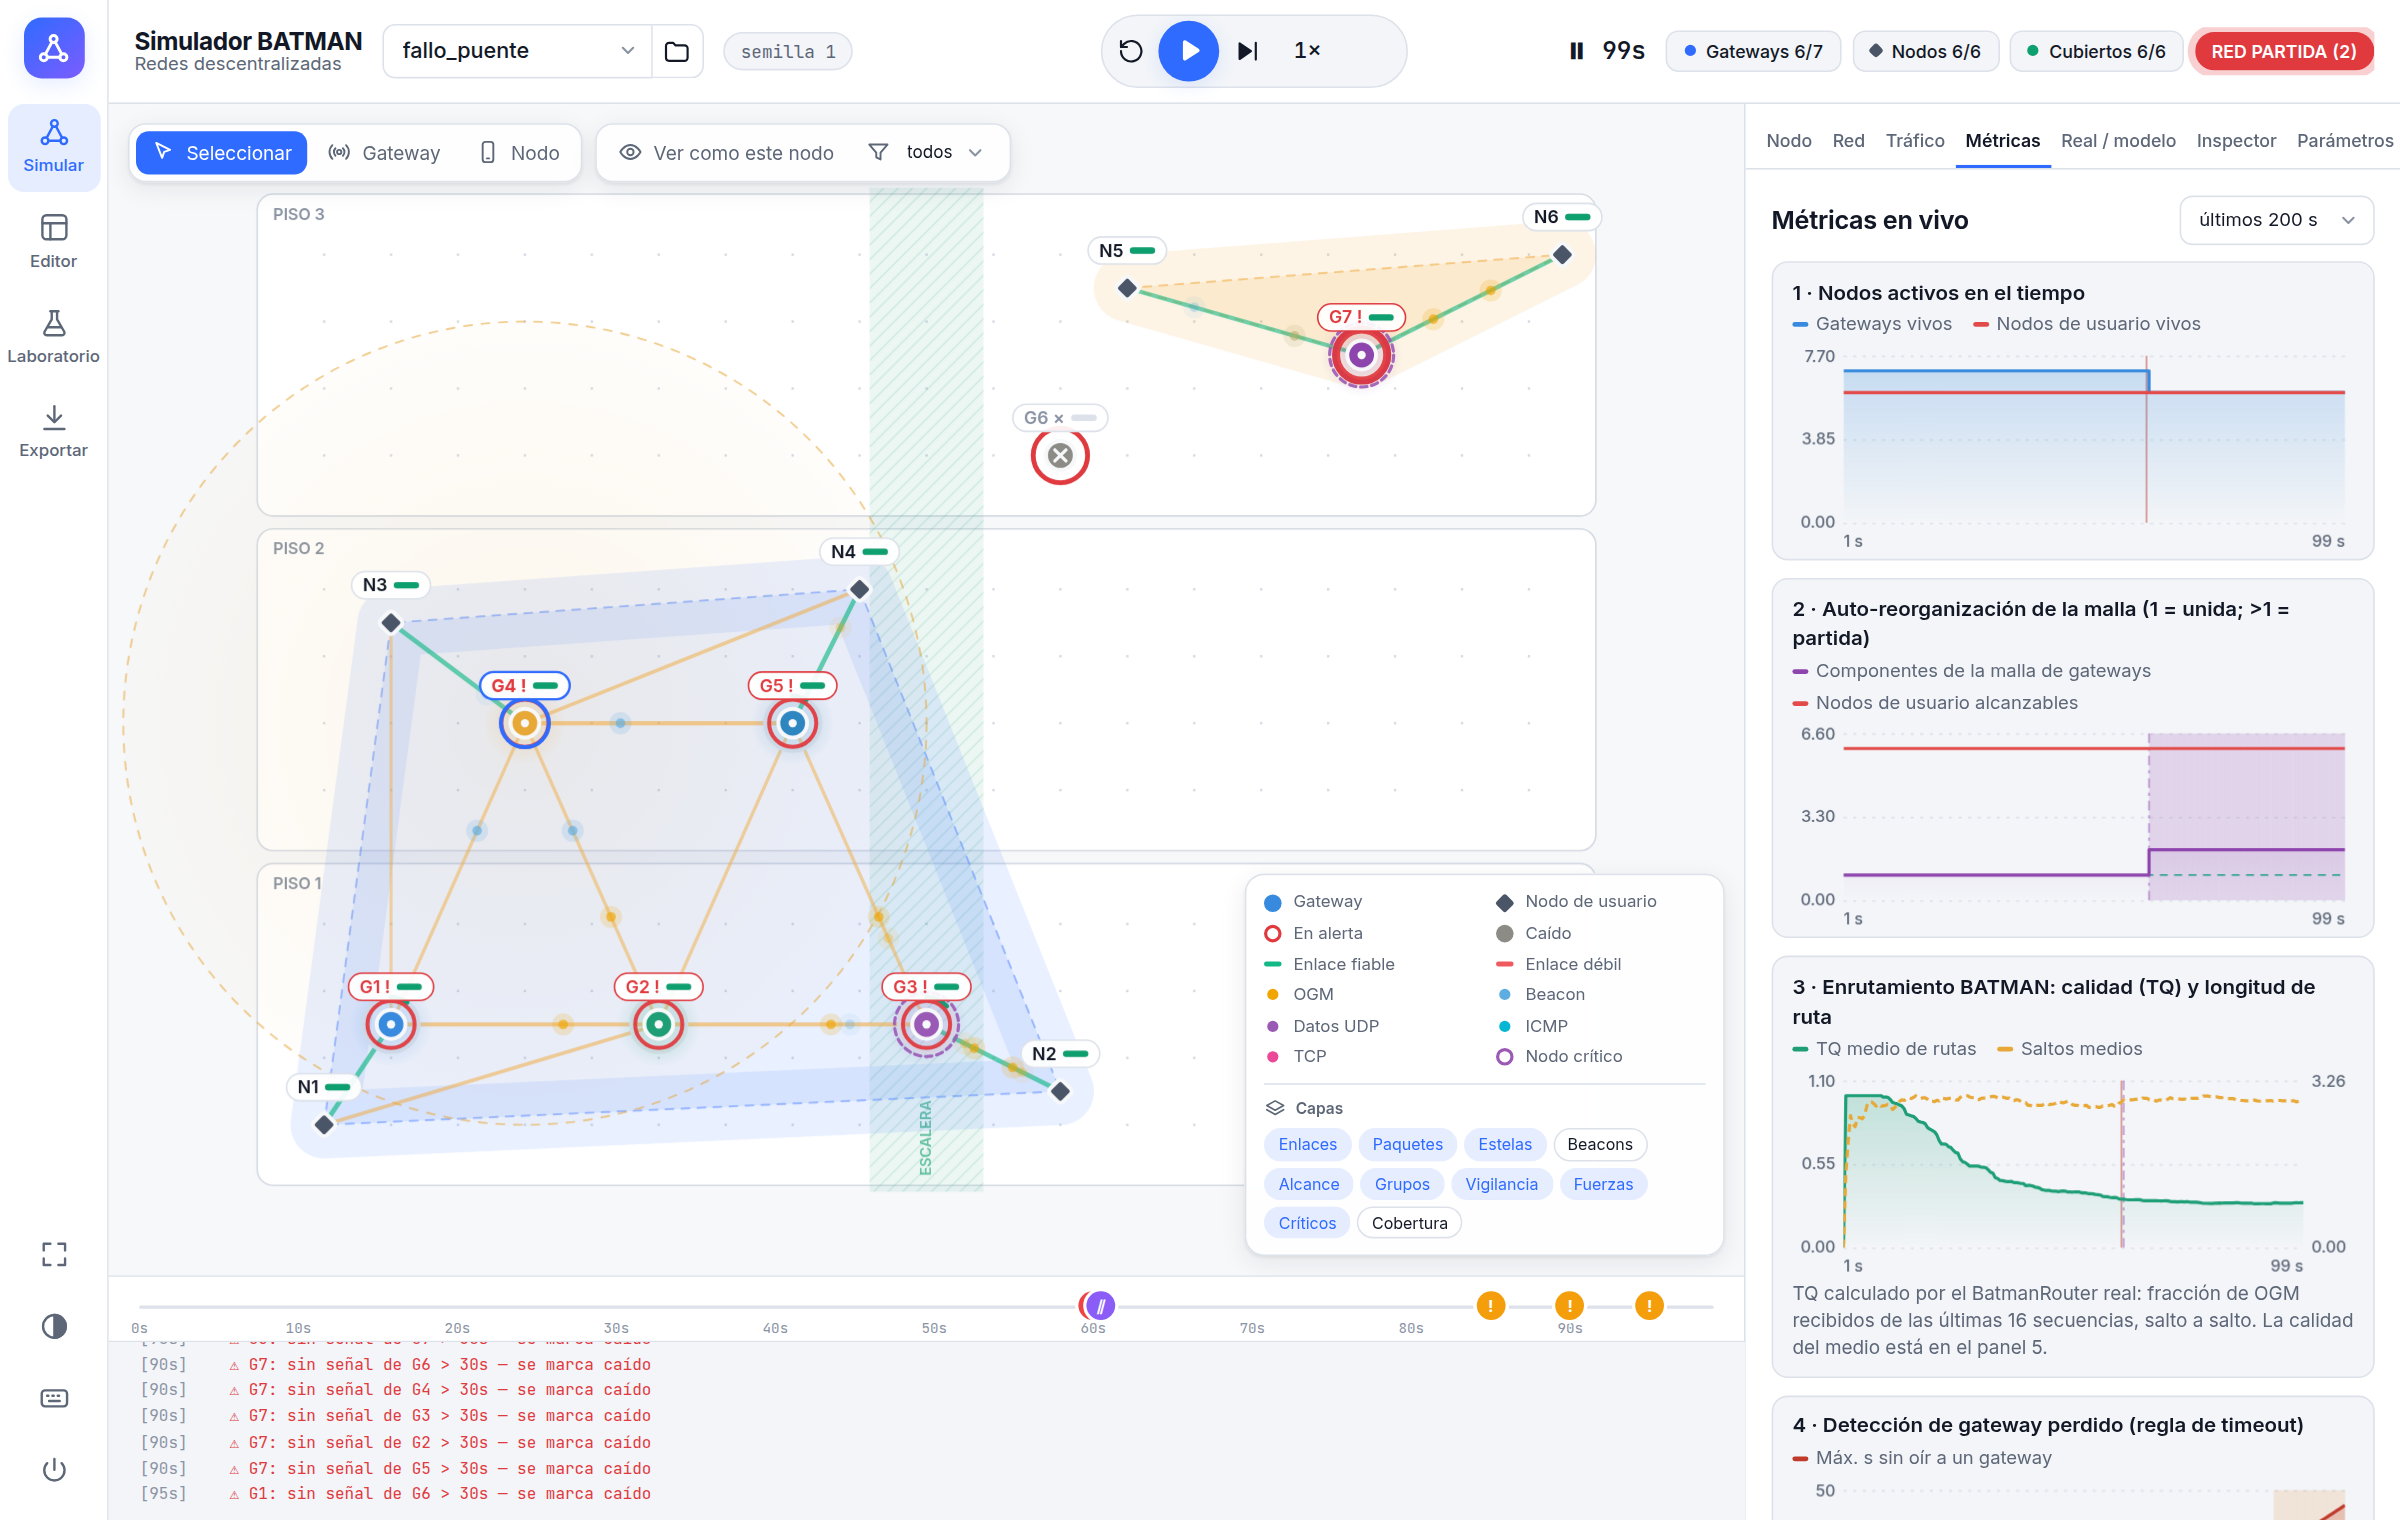
\includegraphics[width=\textwidth, trim=1740 250 0 130, clip]{Images/Cap4/metricas.png}
        \caption{Panel de métricas en vivo}
    \end{subfigure}
    \caption{Dos paneles de la interfaz a los 99~s de la prueba de la caída del puente. (a) A la izquierda, lo que ejecutó el código del nodo (OGM y \textit{beacons} procesados, rutas en las tablas, revisiones de fallos); a la derecha, lo que aportó el modelo: el medio intentó 8783 entregas y completó el 60.5~\%. (b) Gráficas que se actualizan durante la corrida: nodos vivos, número de grupos de la malla (sube de 1 a 2 al caer el puente, zona sombreada) y calidad y longitud de las rutas}
    \label{fig:real-modelo}
\end{figure}

\textbf{Tráfico de datos.} En el panel de la Figura~\ref{fig:trafico} se eligen
el origen, el destino, el tipo de paquete, la cantidad y el intervalo. El panel
muestra cuántos paquetes de cada tipo se enviaron y se entregaron, los flujos
activos y el recorrido de los últimos paquetes, incluida la respuesta de
regreso en ICMP y TCP.

\begin{figure}[htbp!]
    \centering
    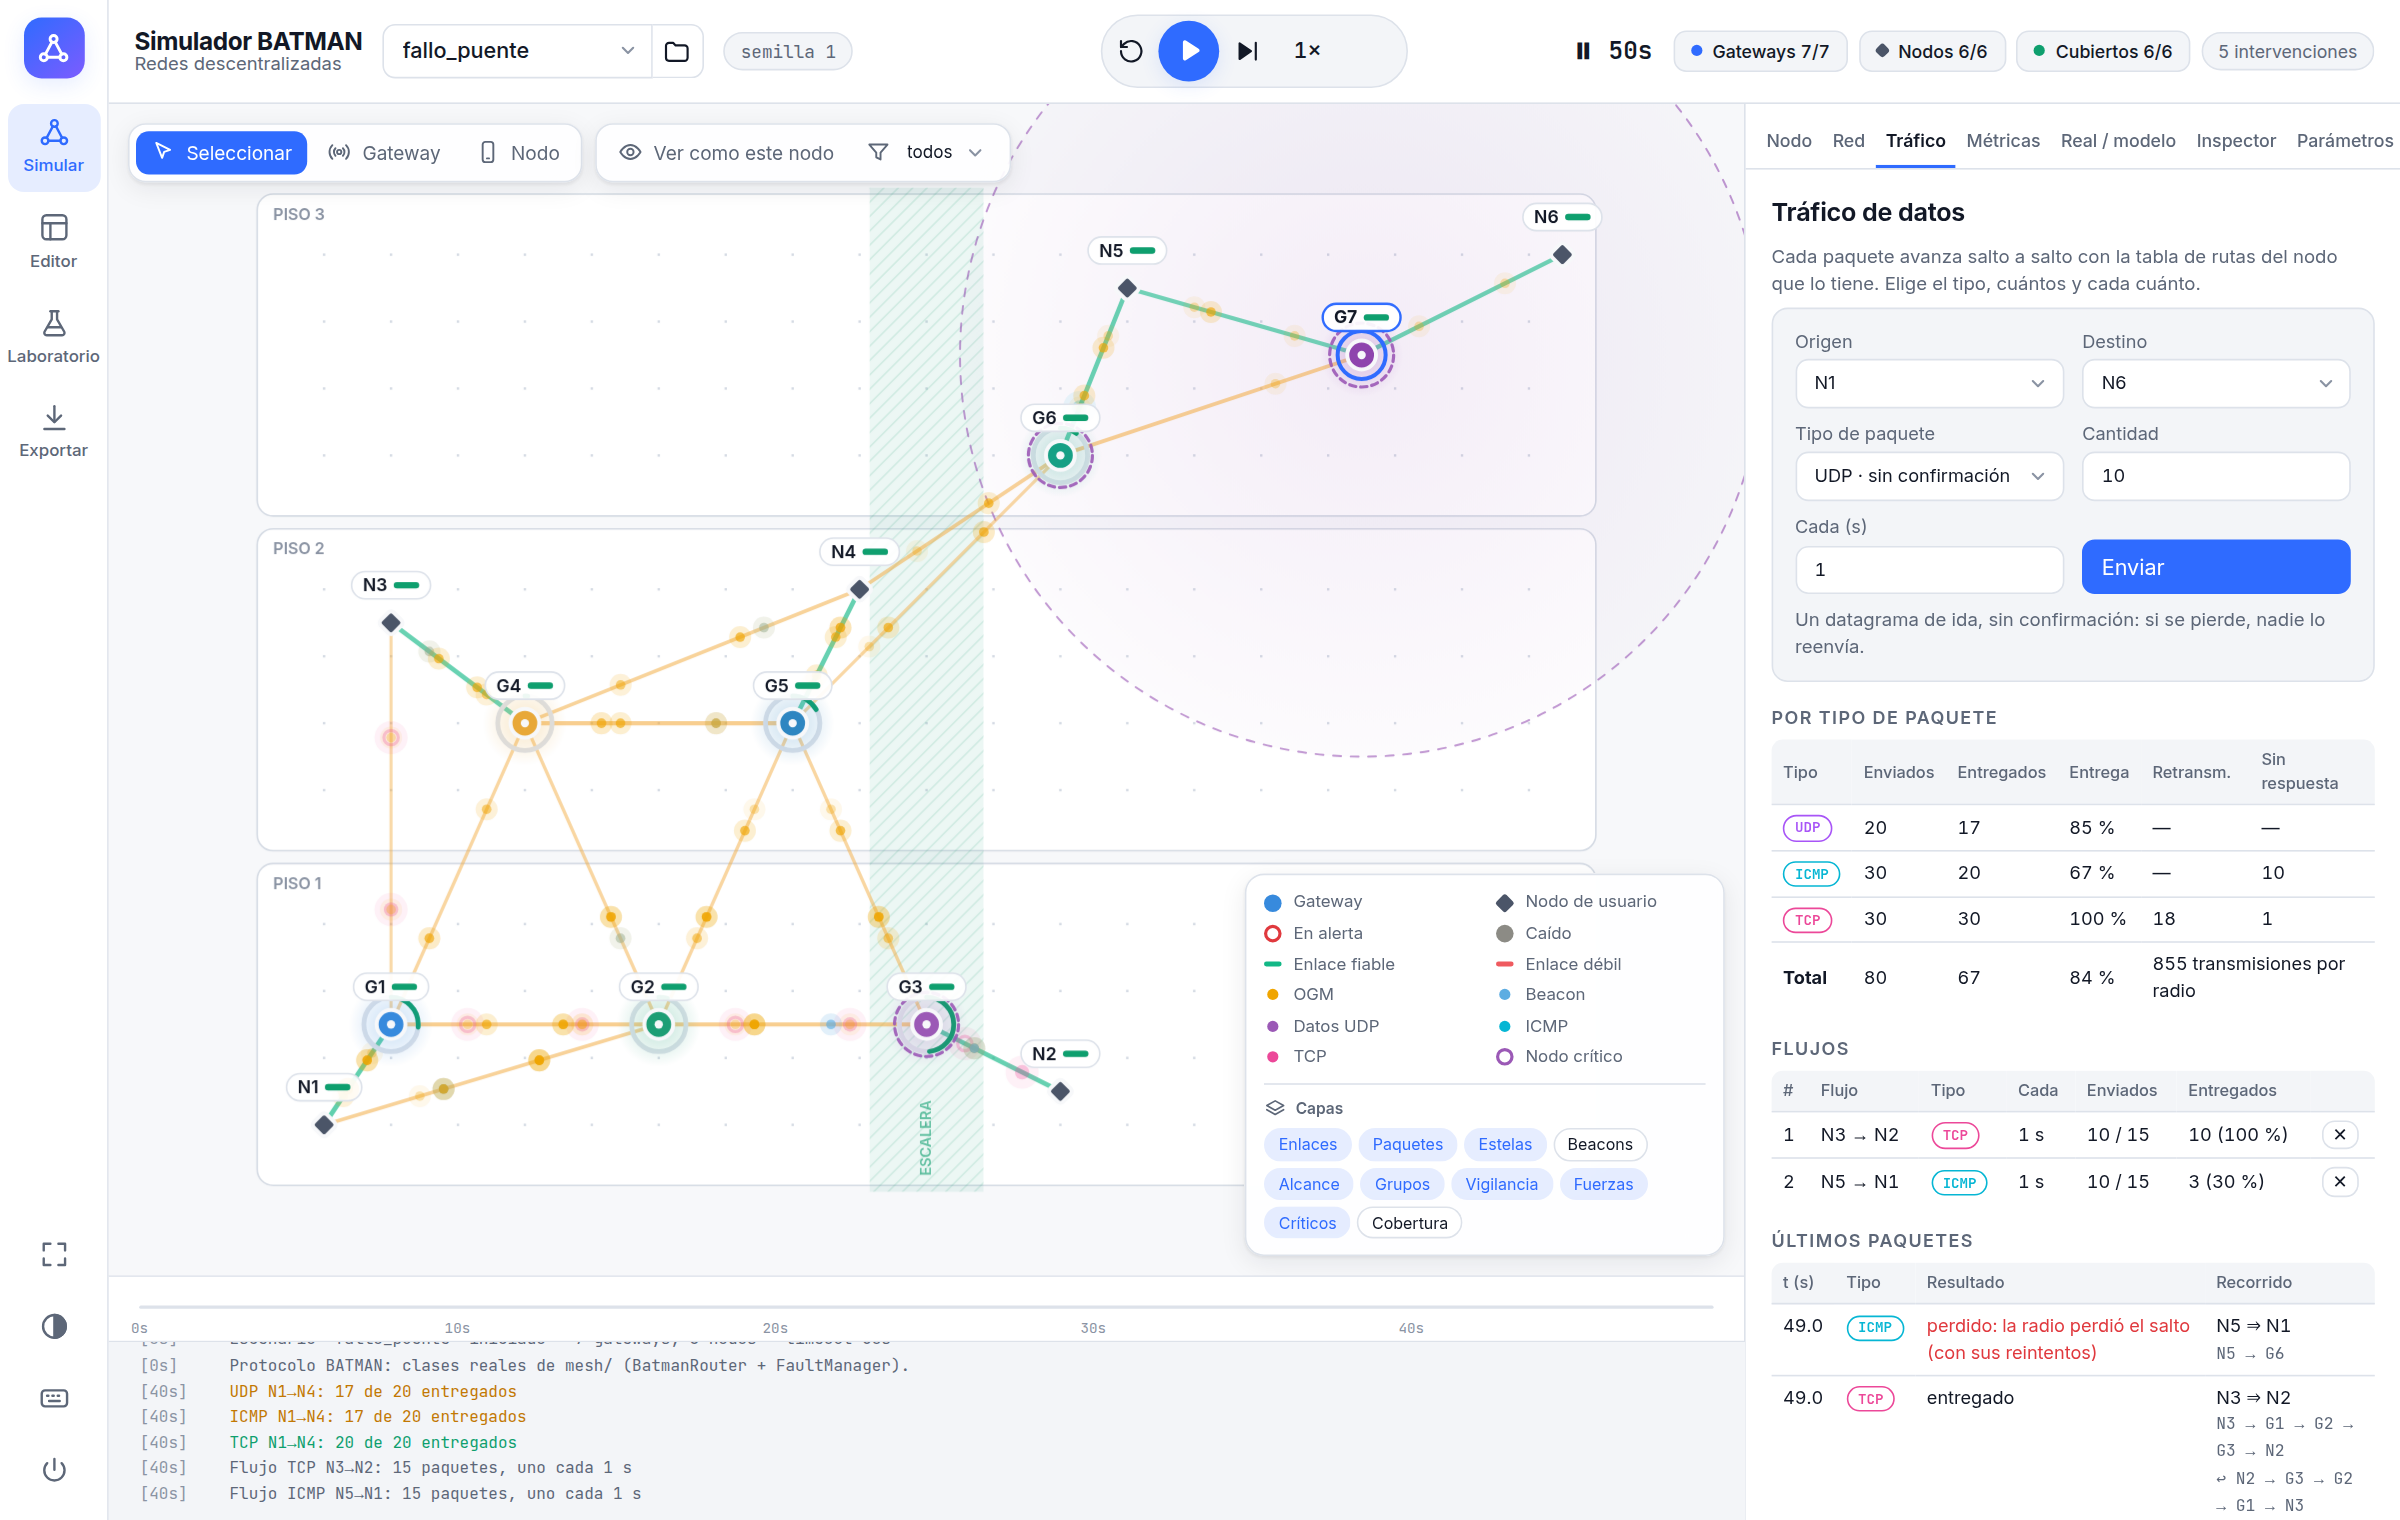
\includegraphics[width=\textwidth]{Images/Cap4/trafico.png}
    \caption{Panel de tráfico a los 50~s de una sesión sobre el despliegue de referencia. Arriba, el formulario para elegir origen, destino, tipo de paquete, cantidad e intervalo. En la tabla ``Por tipo de paquete'' se ve el resultado de enviar 20 paquetes de cada tipo de N1 a N4 y dos flujos adicionales: UDP entregó 17 de 20; ICMP, 20 de 30, con 10 ecos sin respuesta; TCP, 30 de 30, con 18 reenvíos. Abajo, los flujos en curso y los últimos paquetes con su recorrido de ida y de vuelta. En el mapa, los puntos de colores son paquetes en tránsito}
    \label{fig:trafico}
\end{figure}

\textbf{Capas del mapa.} El mapa tiene capas que se encienden y se apagan. La
Figura~\ref{fig:fuerzas} muestra tres de ellas con Gateway móviles: el mapa de
cobertura, los nodos críticos y la decisión de movimiento de cada Gateway.

\begin{figure}[htbp!]
    \centering
    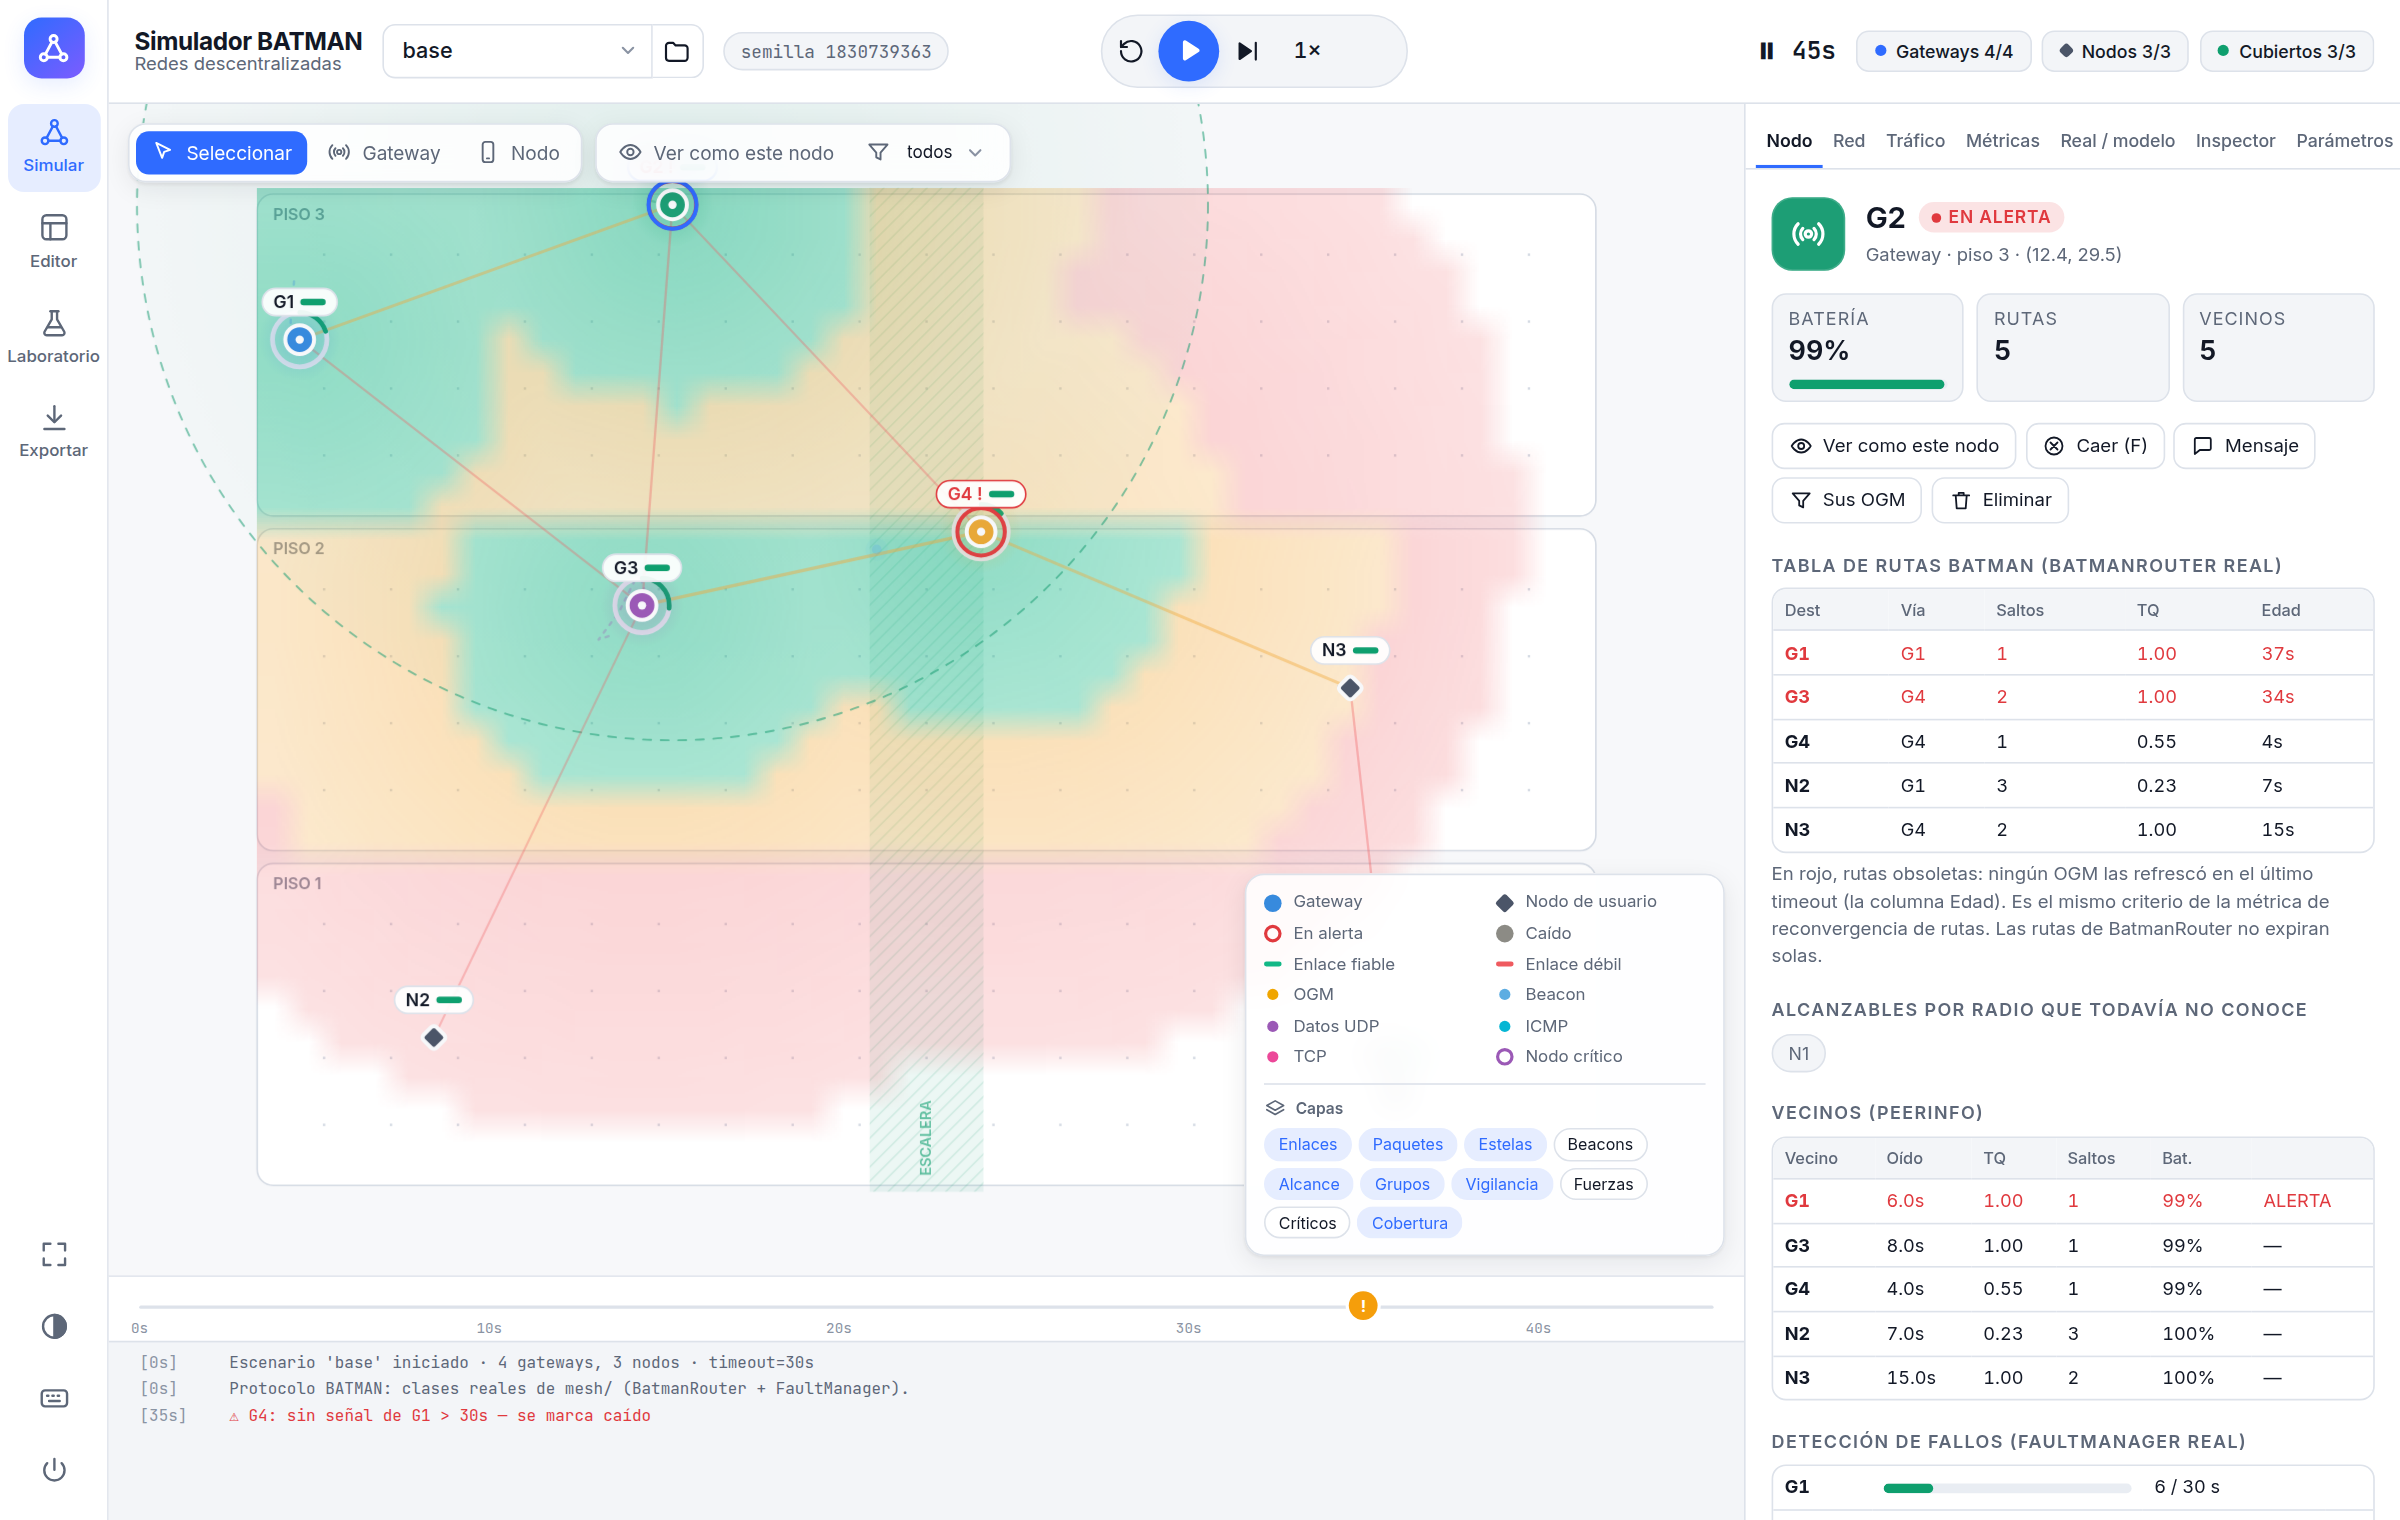
\includegraphics[width=\textwidth]{Images/Cap4/fuerzas_cobertura.png}
    \caption{Capas del mapa con movimiento descentralizado (escenario \texttt{base} a los 45~s). El fondo de colores es el mapa de cobertura: verde donde la señal de algún Gateway es buena, amarillo donde es débil y rojo donde no llega. Los Gateway se han separado desde su posición inicial para cubrir más área; el anillo punteado marca un nodo crítico y el círculo grande, el alcance del Gateway seleccionado (G2), cuya tabla de rutas y vecinos aparece a la derecha}
    \label{fig:fuerzas}
\end{figure}

\textbf{Editor de escenarios y laboratorio.} El editor
(Figura~\ref{fig:editor}a) permite armar un escenario con el ratón y guardarlo
como archivo. El laboratorio (Figura~\ref{fig:editor}b) corre lotes de
escenarios con varias semillas, con los mismos números que la terminal.

\begin{figure}[htbp!]
    \centering
    \begin{subfigure}{0.49\textwidth}
        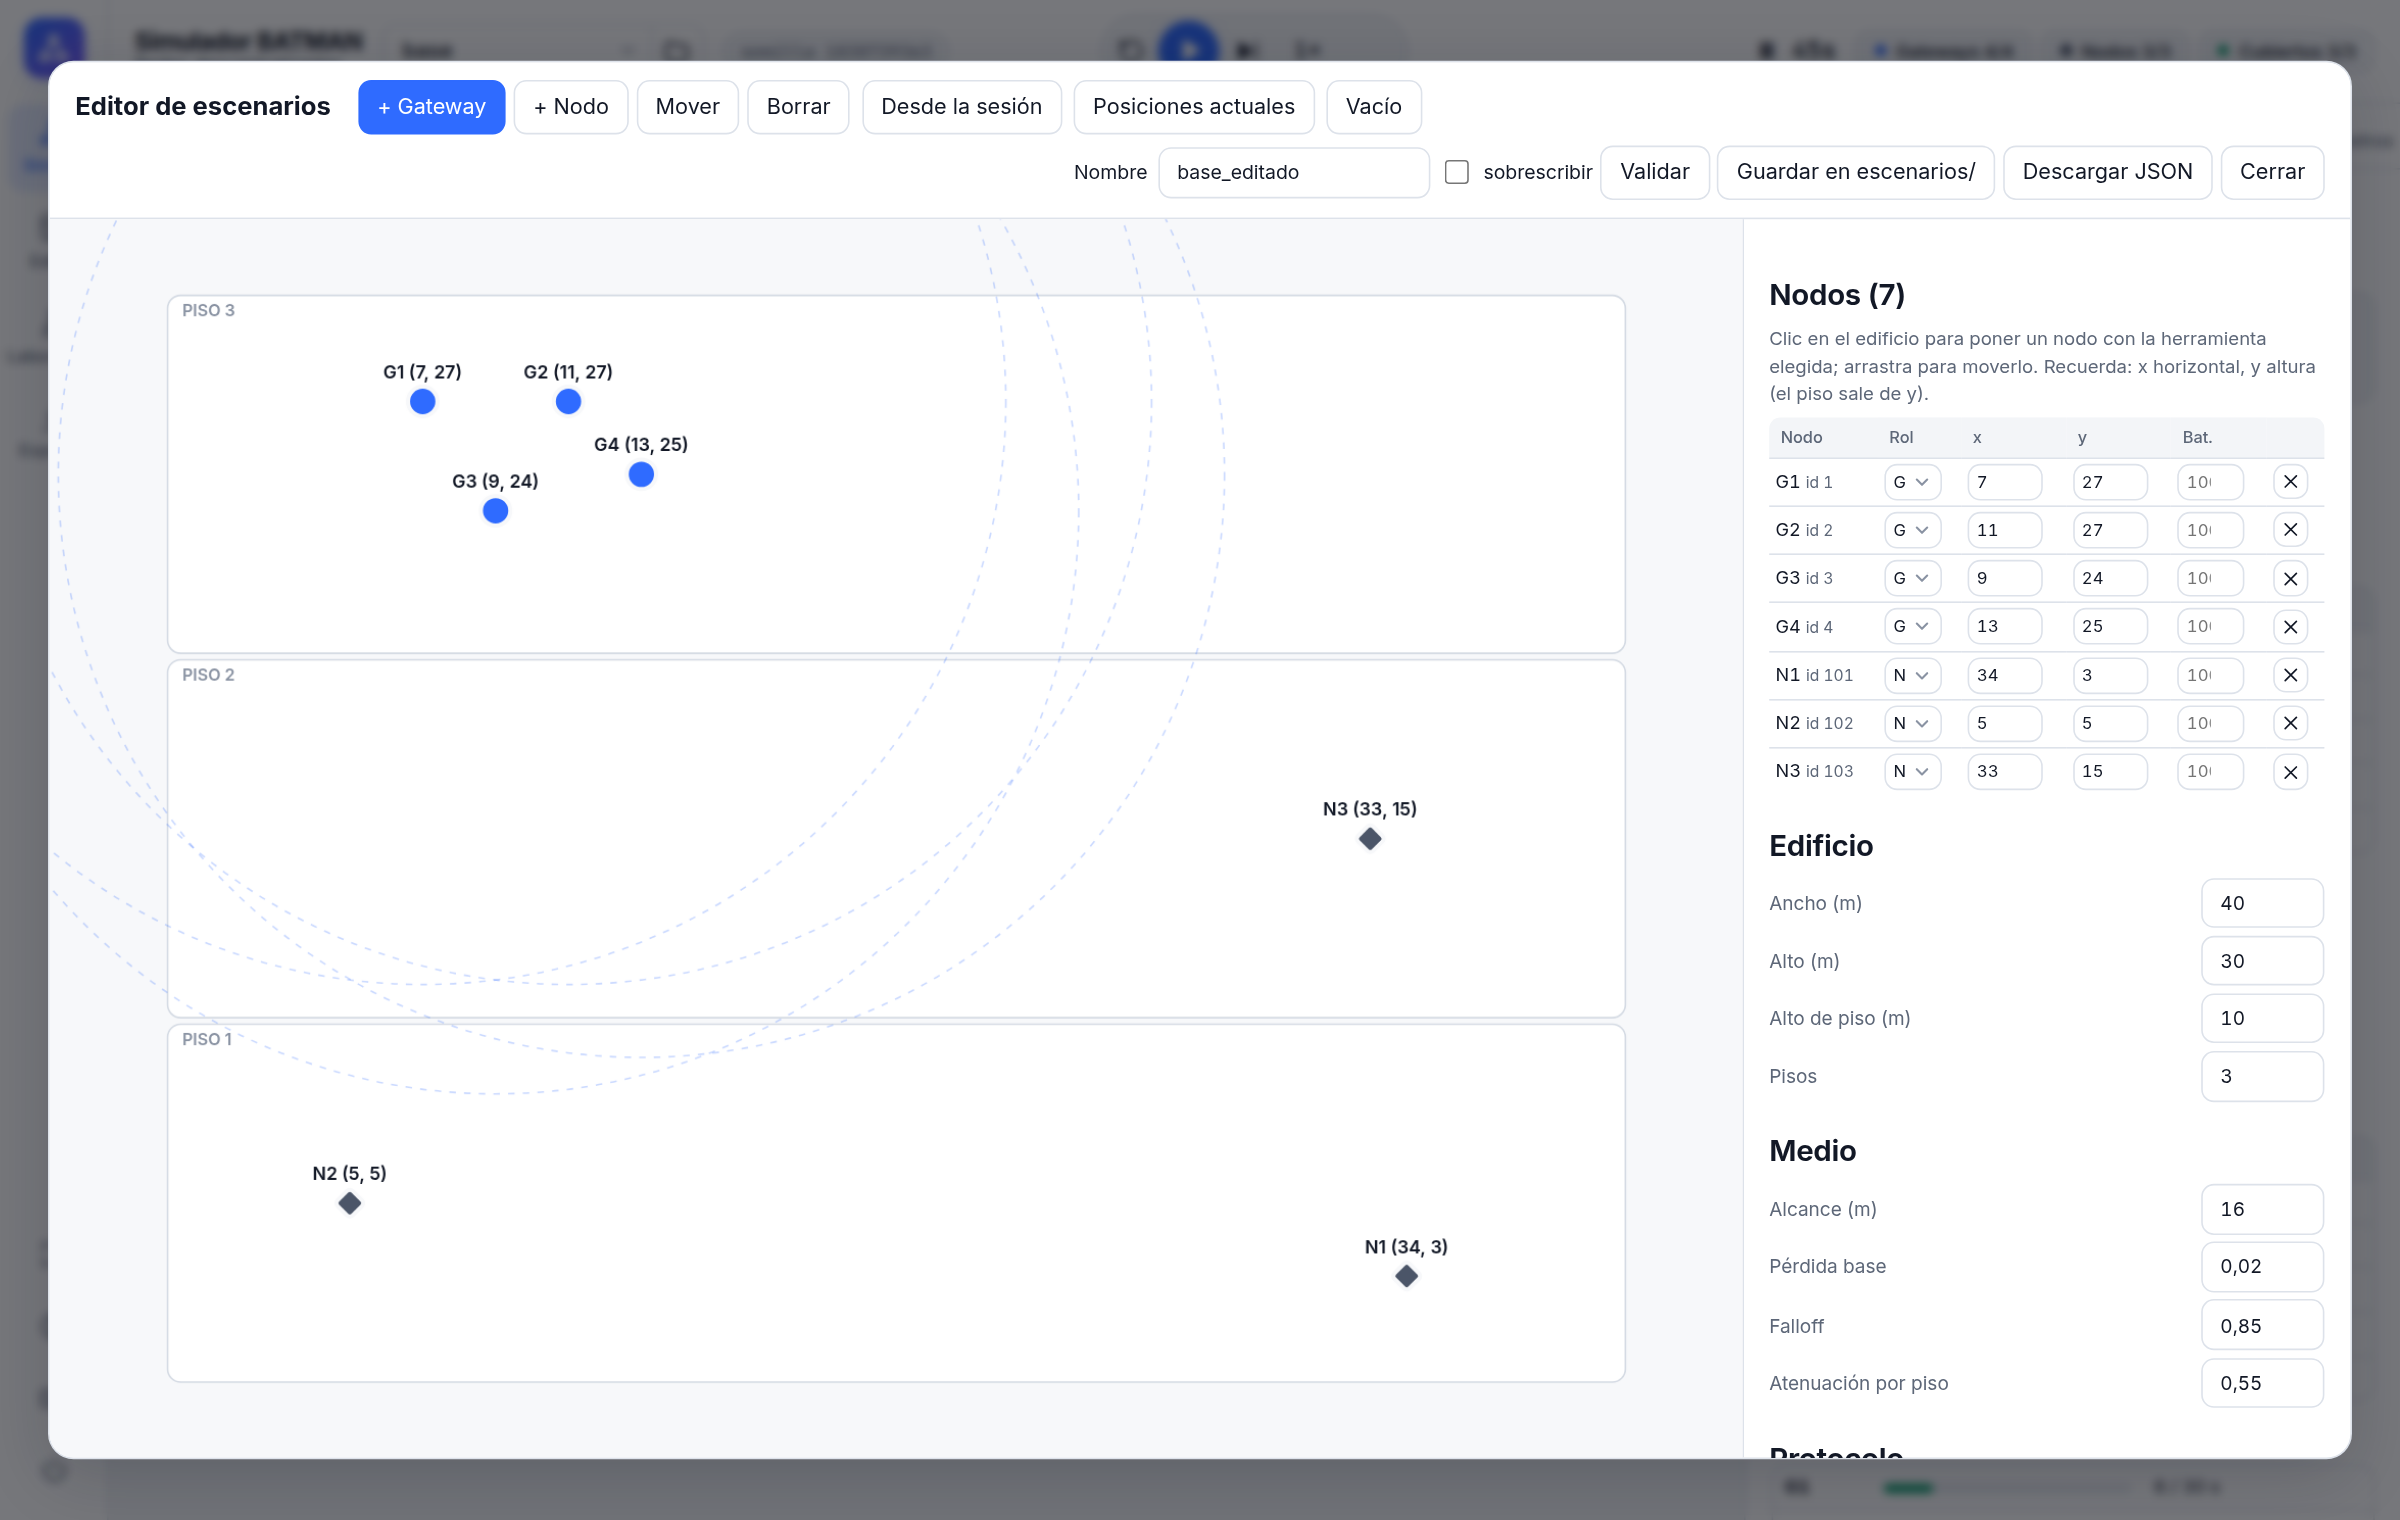
\includegraphics[width=\textwidth]{Images/Cap4/editor.png}
        \caption{Editor de escenarios}
    \end{subfigure}\hfill
    \begin{subfigure}{0.49\textwidth}
        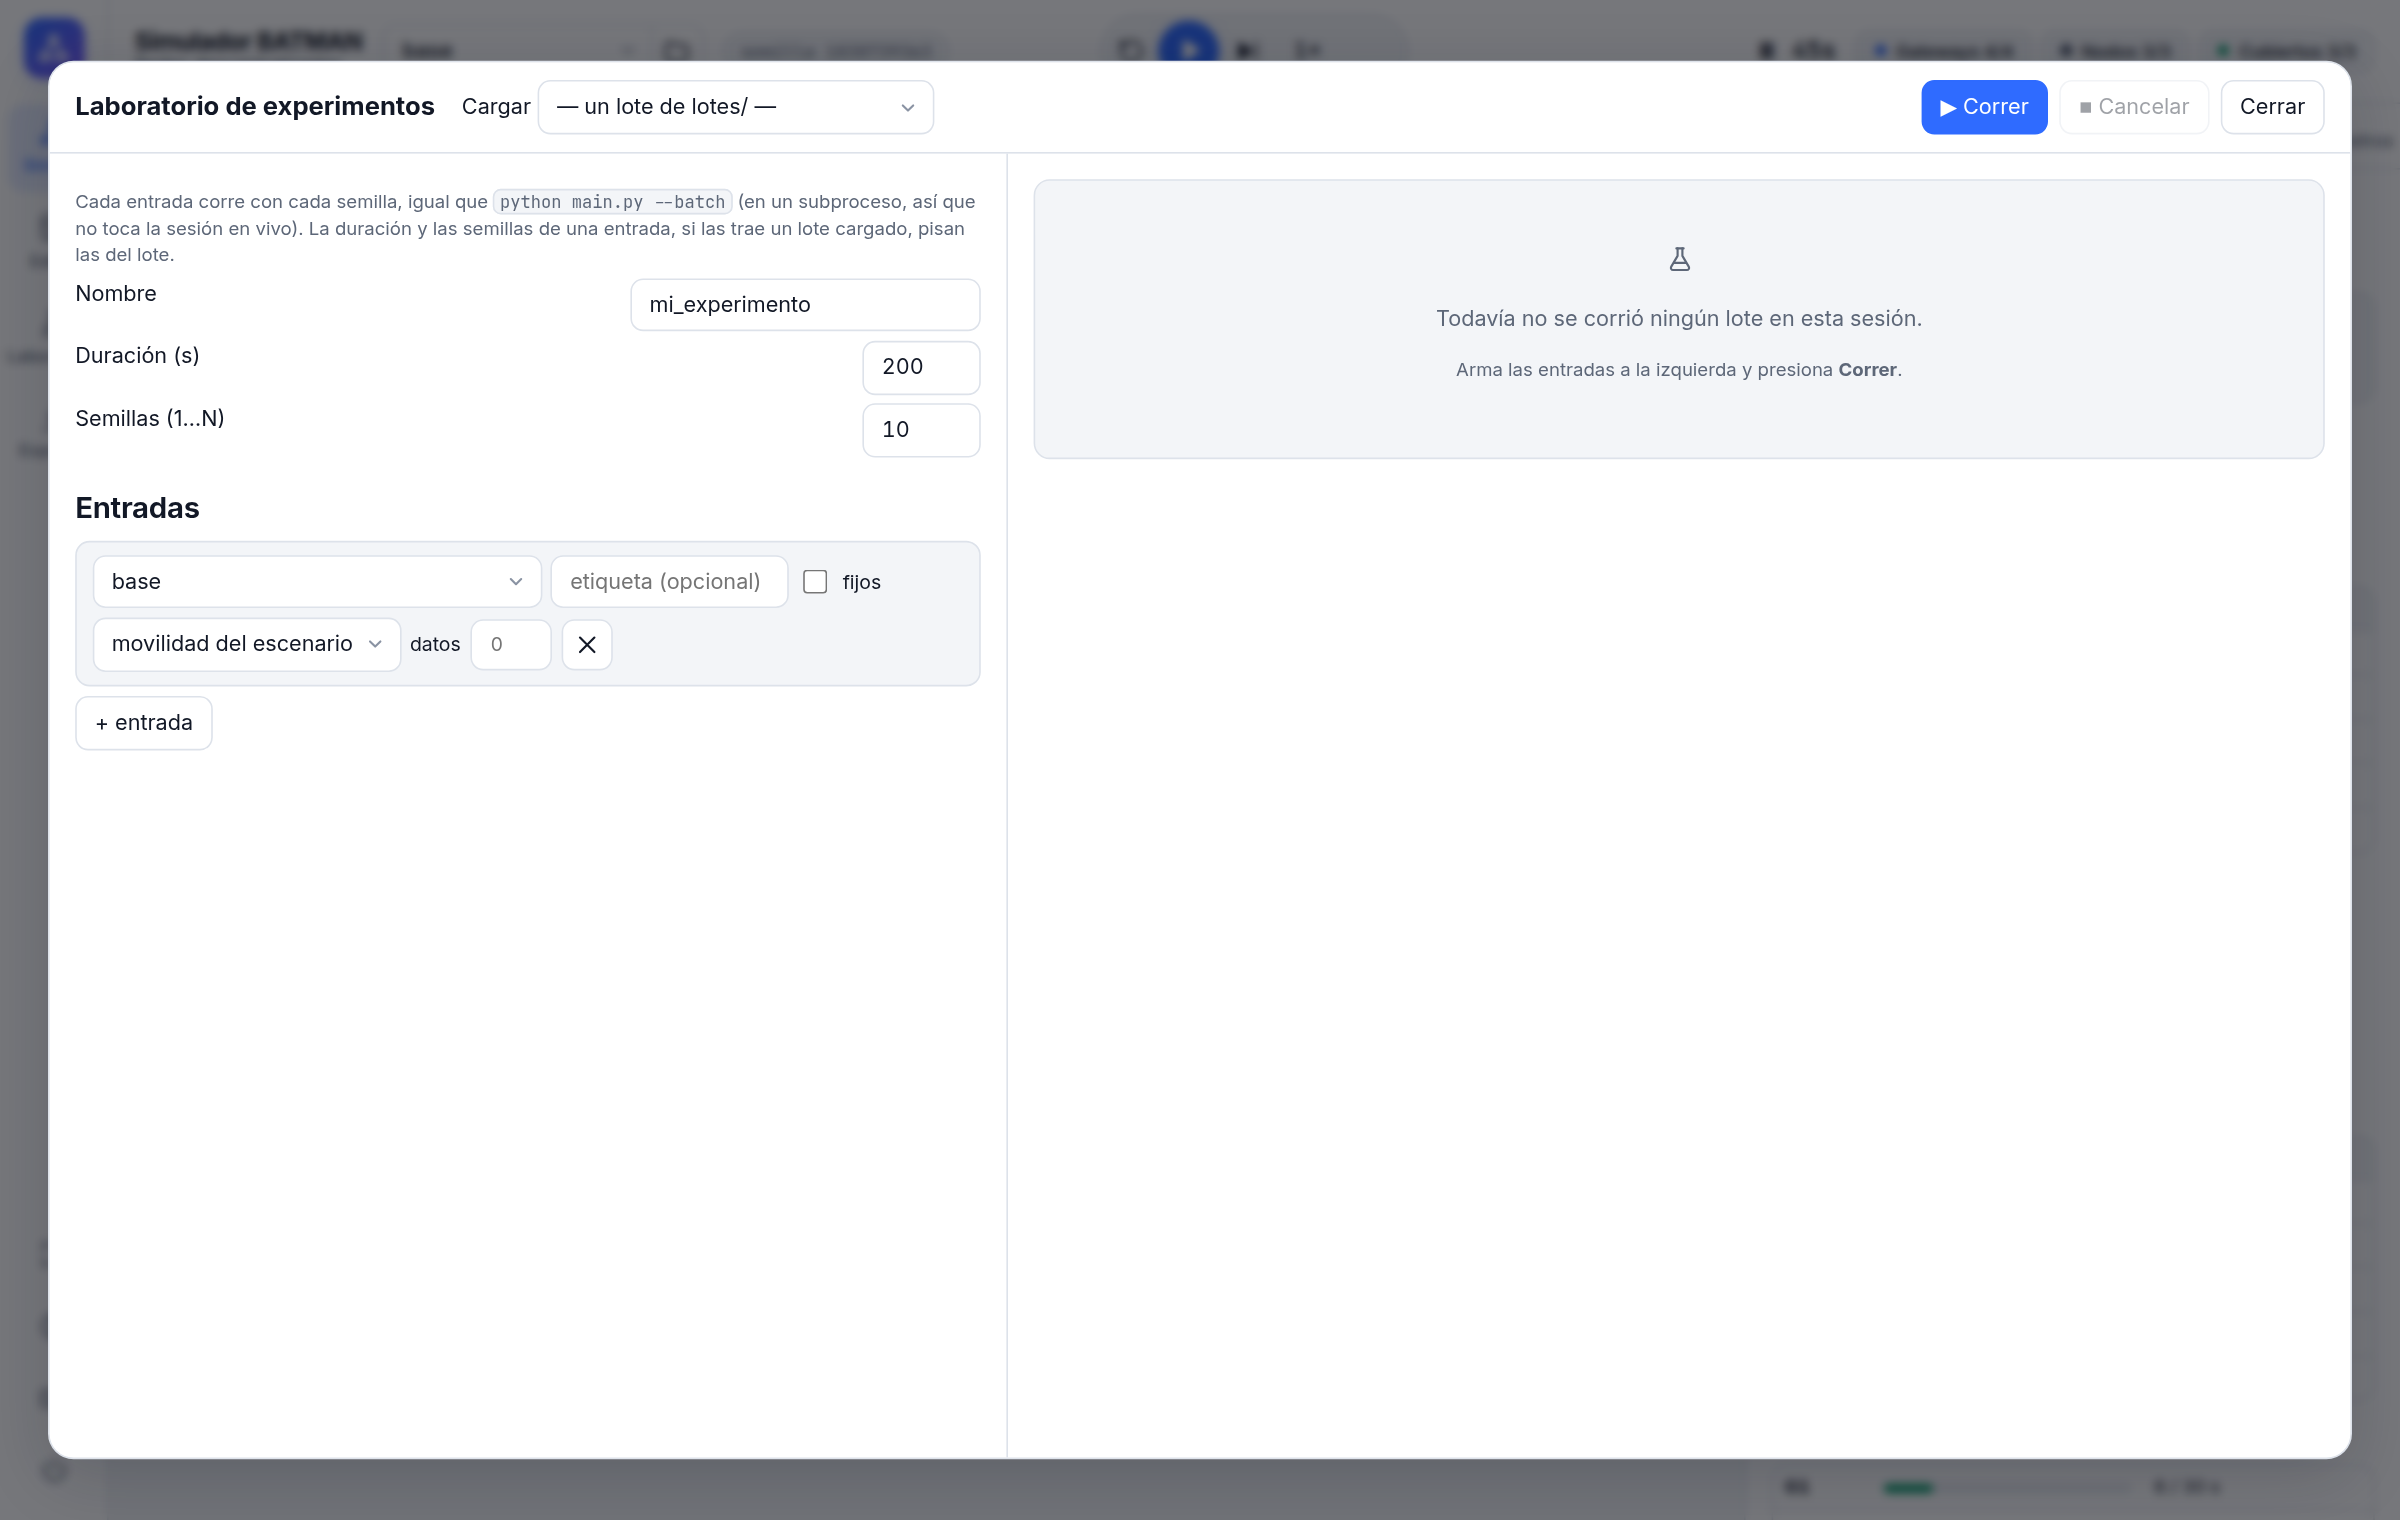
\includegraphics[width=\textwidth]{Images/Cap4/laboratorio.png}
        \caption{Laboratorio de experimentos}
    \end{subfigure}
    \caption{(a) Editor de escenarios: a la izquierda, el edificio donde se ponen y se arrastran los nodos; a la derecha, la lista de nodos y los valores del edificio y del medio. (b) Laboratorio: se indica la duración, el número de semillas y los escenarios que se quieren comparar, y al terminar muestra el promedio de cada métrica}
    \label{fig:editor}
\end{figure}

La Tabla~\ref{tab:interfaz} resume las funciones de la interfaz, la figura que
sirve de evidencia de cada una y el requerimiento que atiende.

\begin{table}[htbp!]
    \centering
    \caption{Funciones de la interfaz, figura que muestra cada una y requerimiento de la Tabla~\ref{tab:requisitos} que atiende}
    \label{tab:interfaz}
    \footnotesize
    \begin{tabular}{|p{4.3cm}|p{5.9cm}|p{1.7cm}|p{1.5cm}|}
        \hline
        \textbf{Función} & \textbf{Qué permite} & \textbf{Evidencia} & \textbf{Req.} \\
        \hline
        Panel de nodo & Ver la tabla de rutas y los vecinos de un nodo & Figura~\ref{fig:interfaz} & R1, R5 \\
        \hline
        ``Ver como este nodo'' & Ver la red solo con lo que sabe un nodo & Figura~\ref{fig:lente} & R4, R5 \\
        \hline
        Matriz de conocimiento & Ver qué sabe cada nodo de los demás & Figura~\ref{fig:matriz} & R5 \\
        \hline
        OGM de un origen, con su TTL & Seguir los mensajes del protocolo salto a salto & Figura~\ref{fig:ogm} & R1 \\
        \hline
        Panel ``Real / modelo'' & Separar lo que hizo el código de lo que aportó el modelo & Figura~\ref{fig:real-modelo}a & R2 \\
        \hline
        Métricas en vivo & Ver la evolución de la red durante la corrida & Figura~\ref{fig:real-modelo}b & R5 \\
        \hline
        Panel de tráfico & Elegir tipo, cantidad e intervalo de los paquetes y ver su recorrido & Figura~\ref{fig:trafico} & R9 \\
        \hline
        Capas de cobertura, críticos y fuerzas & Ver el efecto de la distancia y los pisos, y la decisión de cada Gateway & Figura~\ref{fig:fuerzas} & R3, R4 \\
        \hline
        Caer y recuperar nodos, arrastrarlos y cambiar parámetros & Experimentar sin equipos físicos & Figura~\ref{fig:interfaz} & R8, R10 \\
        \hline
        Editor y laboratorio & Crear escenarios y repetirlos con semillas & Figura~\ref{fig:editor} & R6, R10 \\
        \hline
    \end{tabular}
\end{table}

\subsection{Costo por nodo}
\label{subsec:costo}

La Tabla~\ref{tab:escala} mide la velocidad del simulador con redes de distinto
tamaño en el mismo edificio, con nodos fijos y 6 flujos de datos, en un
computador portátil con un procesador Intel Core i5-1035G1. El costo crece
mucho más rápido que el número de nodos: al medir la corrida de 100 nodos, cerca
del 90~\% del tiempo se fue en procesar y reenviar los OGM, porque al crecer la
red en la misma área todos se oyen con todos y cada OGM se repite muchas veces.
Esto marca el rango de uso de la herramienta: con decenas de nodos corre más
rápido que el tiempo real; con unos 100 nodos juntos, más lento; y no sirve para
miles de nodos sin optimizarla. El requerimiento R7 se cumple entonces solo en
parte: se evita el costo de una máquina virtual por nodo, pero un emulador como
CORE reporta más de un centenar de nodos en tiempo
real~\cite{Ahrenholz2008Core}. La ventaja de esta herramienta frente a la
emulación está en el control, la repetibilidad y las mediciones, no en el
tamaño.

\begin{table}[htbp!]
    \centering
    \caption{Velocidad del simulador según el tamaño de la red (una corrida, semilla 1). La última columna indica cuántos segundos de simulación se calculan en un segundo de reloj: por encima de 1, el simulador va más rápido que el tiempo real}
    \label{tab:escala}
    \footnotesize
    \begin{tabular}{|p{2.4cm}|p{2.4cm}|p{3.0cm}|p{3.2cm}|}
        \hline
        \textbf{Nodos} & \textbf{Gateway} & \textbf{Tiempo por paso (ms)} & \textbf{Segundos simulados por segundo real} \\
        \hline
        14 & 8 & 1.8 & 284.5 \\
        \hline
        25 & 10 & 9.2 & 54.1 \\
        \hline
        50 & 20 & 78.6 & 6.4 \\
        \hline
        100 & 40 & 816.7 & 0.6 \\
        \hline
        200 & 80 & 12\,006 & 0.04 \\
        \hline
    \end{tabular}
\end{table}

\subsection{Diferencias con B.A.T.M.A.N.}
\label{sec:fidelidad}

Conviene precisar qué significa aquí ``código real''. \texttt{BatmanRouter} y
\texttt{FaultManager} son las clases que usa el nodo de red de este proyecto
(\texttt{mesh/node.py}), de modo que lo que se evalúa es esa implementación y
no una copia escrita aparte. Pero esa implementación no es el módulo
batman-adv~\cite{OpenMesh2024Batmanadv}, ni se ha ejecutado en este trabajo
sobre equipos de radio. Las diferencias conocidas con el
protocolo~\cite{Neumann2008Batman} son:

\begin{itemize}
\item \textbf{Reenvío de OGM.} Se reenvía la primera copia de cada mensaje,
llegue por donde llegue. El protocolo solo reenvía la que llegó por el mejor
vecino. Esto produce bucles en las tablas (Sección~\ref{sec:res-protocolo}).
\item \textbf{Vencimiento de rutas.} Las rutas no se borran solas: una ruta por
un vecino caído solo se reemplaza cuando aparece otra mejor. El protocolo borra
al nodo de origen cuando pasa un tiempo sin oírlo.
\item \textbf{Reinicio.} Un nodo que se recupera conserva su número de
secuencia; un arranque desde cero queda fuera del modelo.
\end{itemize}

Durante el desarrollo se corrigieron además tres defectos que afectaban a las
conclusiones: el TQ valía siempre 1.0 porque nunca se registraban los OGM
perdidos, la primera copia de cada mensaje ganaba la ruta sin mirar el TQ, y
una alerta sobre un Gateway lejano nunca se apagaba.

% ════════════════════════════════════════════════════════════════════════
\section{Pruebas}
\label{sec:pruebas}

Las pruebas del simulador son simulaciones: escenarios que cualquiera puede
volver a ejecutar, cada uno con un propósito y un resultado esperado que se
compara con lo que el simulador produce. La Tabla~\ref{tab:experimentos} las
presenta. Las pruebas P1 a P3 comprueban funciones básicas con una corrida que
se puede observar en la interfaz; las pruebas P4 a P9 comparan configuraciones
con 10 semillas cada una, y las pruebas P10 y P11 comprueban propiedades de la
herramienta. Los resultados están en el Capítulo~\ref{cap:resultados}.

{\footnotesize
\begin{longtable}{|p{0.6cm}|p{2.6cm}|p{4.5cm}|p{5.3cm}|}
    \caption{Pruebas de simulación: nombre, propósito y resultado esperado de cada una\label{tab:experimentos}}\\
    \hline
    \textbf{N.º} & \textbf{Nombre} & \textbf{Propósito} & \textbf{Qué se espera} \\
    \hline
    \endfirsthead
    \hline
    \textbf{N.º} & \textbf{Nombre} & \textbf{Propósito} & \textbf{Qué se espera} \\
    \hline
    \endhead
    P1 & Formación de la malla & Comprobar que los nodos se descubren y arman sus tablas de rutas sin ayuda & A los 30~s, casi todos los pares de nodos conectados por radio tienen una ruta \\
    \hline
    P2 & Propagación de un OGM & Comprobar que los mensajes del protocolo se reenvían salto a salto & El TTL de las copias baja en uno por cada salto desde el origen \\
    \hline
    P3 & Tipos de paquete & Comparar la entrega de UDP, ICMP y TCP con el mismo tráfico (lote \texttt{tipos\_paquete}) & ICMP entrega menos que UDP, porque necesita ida y vuelta; TCP entrega más que UDP, con más transmisiones \\
    \hline
    P4 & Fallos con Gateway fijos & Medir cómo responde la malla a la caída de un Gateway redundante, de un puente, de uno de borde y a una cascada de caídas (lote \texttt{capitulo5\_fallos}) & El redundante no afecta la cobertura; el puente parte la malla 90~s; el de borde deja a N6 sin cobertura (0.9375); la cascada baja la cobertura a 0.736 \\
    \hline
    P5 & Los mismos fallos con Gateway móviles & Medir si la malla se adapta sola cuando los Gateway pueden moverse (lote \texttt{capitulo5\_fallos\_movil}) & La malla pasa menos tiempo partida que con Gateway fijos \\
    \hline
    P6 & Modos de movimiento & Comparar el movimiento descentralizado con los dos modos centralizados en 5 escenarios (lote \texttt{movilidad}) & El modo descentralizado mantiene la malla unida con una cobertura cercana a la de los centralizados \\
    \hline
    P7 & Movimiento con tráfico & Medir qué significan esas diferencias para los paquetes de datos, en 3 escenarios con 6 flujos (lote \texttt{movilidad\_datos}) & El modo que conecta a más nodos entrega más paquetes \\
    \hline
    P8 & Fallos al azar y dirigidos & Comparar dos caídas al azar con dos dirigidas al nodo más crítico (lote \texttt{robustez}) & Los fallos dirigidos hacen más daño que los fallos al azar \\
    \hline
    P9 & B.A.T.M.A.N. e inundación & Comparar el protocolo con la inundación en campo abierto y en el edificio (lote \texttt{generalidad}) & La inundación entrega más a cambio de más transmisiones \\
    \hline
    P10 & Repetibilidad & Comprobar que la misma semilla da la misma corrida, también en otro computador & Las tablas de resultados salen idénticas \\
    \hline
    P11 & Tamaño de la red & Medir hasta cuántos nodos es práctico el simulador & El tiempo de cálculo crece con el número de nodos (Tabla~\ref{tab:escala}) \\
    \hline
\end{longtable}
}

En las pruebas de fallos (P4 y P5), el Gateway redundante (G2), el puente (G6) y
el de borde (G7) se caen a los 60~s y vuelven a los 150~s. En la cascada se caen
G6 a los 60~s, G7 a los 100~s y G3 a los 140~s, y no vuelven. Las corridas duran
entre 200 y 300~s simulados.

\subsection{Ejemplo de una prueba: la caída del puente}
\label{subsec:ejemplo-prueba}

Para mostrar cómo se lee una prueba, se toma una corrida de la prueba P4: la
caída del Gateway puente con la semilla 1. Se ejecuta con la orden:

\begin{verbatim}
python main.py --headless --duracion 240 --seed 1 \
    --config escenarios/fallos/fallo_puente.txt
\end{verbatim}

El resultado esperado se puede calcular antes de simular: G6 es el único enlace
con el piso 3 y está caído de los 60~s a los 150~s, de modo que la malla debe
estar partida exactamente 90~s; y como cada parte conserva algún Gateway, los
seis usuarios deben seguir cubiertos. La Tabla~\ref{tab:corrida-puente} muestra
lo que entrega el simulador al terminar, y la Figura~\ref{fig:interfaz} muestra
la misma corrida en la interfaz a los 99~s: la red partida en dos y los seis
usuarios cubiertos. Las dos cosas coinciden con lo esperado.

\begin{table}[htbp!]
    \centering
    \caption{Métricas de una corrida de la prueba de la caída del puente (escenario \texttt{fallo\_puente}, 240~s simulados, semilla 1), tal como las entrega el simulador al terminar}
    \label{tab:corrida-puente}
    \footnotesize
    \begin{tabular}{|p{7.4cm}|p{2.0cm}|p{4.2cm}|}
        \hline
        \textbf{Métrica} & \textbf{Valor} & \textbf{Qué se esperaba} \\
        \hline
        Tiempo con la malla partida (s) & 90.0 & 90 (lo que dura la caída) \\
        \hline
        Cobertura media de los Nodos de usuario & 1.000 & 1 (nadie queda aislado) \\
        \hline
        Nodos de usuario alcanzables al final & 6 & 6 \\
        \hline
        Gateway vivos al final & 7 & 7 (G6 vuelve) \\
        \hline
        Grupos de la malla al final & 1 & 1 (se reunifica) \\
        \hline
        Reconvergencia de rutas (s) & 7.5 & Unos pocos periodos de OGM \\
        \hline
        Alertas de Gateway perdido & 22 & Varias: los demás dejan de oír a G6 \\
        \hline
        Instante de la primera alerta (s) & 85.0 & Entre 60 y 90 (límite de 30~s) \\
        \hline
        TQ medio de las rutas & 0.344 & Sin valor esperado \\
        \hline
        Saltos medios por ruta & 2.83 & Sin valor esperado \\
        \hline
        Tasa de entrega del radio & 0.604 & Sin valor esperado \\
        \hline
        Exactitud del conocimiento de rutas & 0.912 & Menor que 1 durante la partición \\
        \hline
        Pares con ruta fantasma / faltante & 0.038 / 0.050 & Mayores que 0 durante la partición \\
        \hline
        Nodos críticos, promedio & 2.62 & Sin valor esperado \\
        \hline
    \end{tabular}
\end{table}

\subsection{Comprobaciones automáticas del código}

Además de las pruebas de simulación, el repositorio incluye 390 comprobaciones
automáticas, que se ejecutan con una sola orden y avisan si un cambio en el
programa alteró algo que ya funcionaba. No son el tema de esta sección; su
detalle está en el Anexo B.
